\chapter{Grover's Search Algorithm}
It is the second most famous quantum algorithm after Shor's algorithm. It doesn't prove exponential speed up, but only a quadratic speedup, yet it is much more widely applicable than Shor's algorithm.

Suppose you are given a map containing many cities, and wish to determine the shortest route passing through all the cities on the map. A simple algorithm to find this route is to search all possible routes through the cities, keeping a running record of which route has the shortest length. On a classical computer, if there are N possible routes, it obviously takes $\mathcal{O}(N)$ operations to determine the shortest route using this method. Remarkably, there is a quantum search algorithm, sometimes known as Grover's algorithm, which enables this search method to sped up substantially, requiring only $\mathcal{O}(\sqrt{N})$ operations. Moreover, the quantum search algorithm is general in the sense that it can be applied far beyond the route-finding example just described to sped up many (though not all) classical algorithms that use search heuristics.

Three main applications of quantum search algorithm are: Quantum counting, speed-up of NP-complete problems, and search of unstructured databases. Here, we also show the optimality of grover's algorithm, i.e. no better search algorithm exists to do even better than a square root speedup. This speed limit applies to most unstructured problems.

\section{The Problem Definition}
\begin{definition}
    \textbf{The Search Problem} For convenience let, $N = 2^n$, we are given an arbitrary $x \in \{0, 1\}^n$.
    Suppose we have a function
    \[
        f:\{0,1\}^n \rightarrow \{0,1\}
    \]
    that is implemented by a reversible transformation (Oracle) $U_f$ in the usual way in the computational basis as:
    \[
        U_f\ket{x}\ket{a}=\ket{x}\ket{a\oplus f(x)}
    \]
    for all $x \in \{0,1\}^n$ and $a \in \{0,1\}$, $\oplus$ denotes addition modulo $2$ and $a$ is a single qubit which is flipped if $f(x)=1$, and is unchanged otherwise. (We can build a quantum circuit for $U_f$ given a Boolean circuit for $f$ at a cost linear in size of boolean circuit). Here, we assume that we are supplied with a quantum oracle - a black box. The problem of search is to simply find a string 
    $ x \in \{0,1\}^n$ such that $f(x)=1$, or to conclude that no such $x$ exists if $f$ is identically 0. 

    This is also called as unstructured search problem because f is arbitrary i.e. there is no promise and we can't rely on it have a structure that makes finding solutions easy. The foal of the algorithm is to find a solution to the search problem, using the smallest possible number of applications of the oracle.
    \begin{remark}Here, we assume that the we can easily evaluate this function $f$ (function can be computed efficiently). That is, maybe we have a boolean circuit whose size is poly(n). This does not restrict the function to be simple. It can be complex and may not have a simple form. This is a \textit{NP-complete} problem. 
    \end{remark}
\end{definition}

\section{The Classical Solution}
Note that the searching problem is completely unstructured. There are no promises on the function $f$, so it is not possible to use binary search or any other fast searching methods to efficiently solve the problem classically. The best classical algorithm for solving the above search problem is Linear search (a \textbf{deterministic algorithm}) and in the worst case it would require $N=2^n$ queries to the black box (to distinguish the case where $f$ is identically 0 from any of the cases where there is a single $x$ for which $f(x)=1$). Thus, $\mathcal{O}(N)$ time complexity. (Here we have assumed that the cost of evaluating $f$ is the one that dominates the computation and hence we talk about the umber of queries to the function $f$ in order to evaluate the time complexity.)

Probabilistically, a best strategy for an algorithm that makes k queries is to simply choose k distinct values of $x$ and to query the black-box at these k values. Then the probability that the $k$ queries contain the solution $x$ will be given by:
\[
Pr= \frac{\binom{N-1}{k-1}}{\binom{N}{k}}=\frac{k}{N}
\]
where $N=2^n$, the number of ways in which our selection contains the solution (in this case we assume that there is a single value fo $x$ for which $f(x)=1$) is choosing the solution (1 way) times choosing $k-1$ from $N-1$ which is $\binom{N-1}{k-1}$ and the total number of ways of possible selections are $\binom{N}{k}$. Thus, the probability $\frac{\binom{N-1}{k-1}}{\binom{N}{k}}=\frac{k}{N}$. Now for the probability that out algorithm succeeds in finding $x$ with probability at least $1-\epsilon$ is,
\[
\frac{k}{2^n} \geq 1-\epsilon
\]
On solving, we get, $k\geq (1-\epsilon)2^n$ number of queries to the oracle. Thus, for constant error we need $\Omega(2^n)=\Omega(N)$ queries to solve the problem.

In the case, when there are multiple solutions (say $a$) and we are interested in designing a probabilistic classical algorithm that succeeds in finding all the solutions with probability at least $1-\epsilon$ is given as follows:
\[
Pr(\text{selecting all the solutions}) = \frac{\binom{N-a}{k-a}}{\binom{N}{k}} = \frac{k(k-1)\ldots (k-a+1)}{n(n-1)\ldots (n-a+1)}
\]
The probability of selecting at least one of the correct solution can be similarly extended.
\textbf{In contrast, the Grover's algorithm will solve the problem using $\mathcal{O}(\sqrt{2^n})$ i.e. $\mathcal{O}(\sqrt{N})$ queries and $\mathcal{O}(\sqrt{N}\log N)$ other gates (the number of gates can be reduced a bit further)}.

\begin{importantnote}
    The problem can be thought of as a table of size N, where exactly one element has value 1, and all others are 0. Searching an item in an unsorted table or array of size N costs a classical computer $\mathcal{O}(N)$ running time. If N is large, this is like searching for a needle in a haystack. This Quantum algorithm for search was proposed by Lov Grover in 1995 that consults the table only $\mathcal{O}(\sqrt{N})$ times.

    In contrast to algorithms like quantum factoring which provide exponential speedups, the search algorithm only provides a quadratic improvement. The same technique used in this algorithm can be used to speedup algorithms for NP-complete problems.

    It is natural to wonder whether there are even faster quantum algorithms for search. However, it turns out that  the quadratic speedup is optimal. This was proved in 1994. Any quantum algorithm for search must consult the table at least some constant times $\sqrt{N}$ times. In this, we have assumed \textit{unique search problem} i.e. This is all assuming that there is only one element that has value 1 and all others have value 0. In case of \textit{multiple solutions} i.e. if there are more than one elements with value 1, then the Grover's algorithm can be modified, and in that case the Complexity becomes $\mathcal{O}(\sqrt{\frac{N}{M}})$, where M is the number of elements with value 1 and N is the total number of elements ($N=2^n)$.
\end{importantnote}
\section{The Quantum Solution: Grover's Algorithm}
Here, we assume the problem to be a Query problem. Thus, the boolean function $f$ implemented on a classical circuit can be converted to a Quantum circuit fro implementing a Query operation using the concepts of reversible computation as explained in section \ref{sec:Oracles}.
\subsection{Idea of the Algorithm}
Just a reminder, we can check whether $x$ is a solution to our problem by preparing $\ket{x}\ket{0}$, applying the oracle, and checking to see if the oracle qubit has flipped to $\ket{1}$. The best way to describe the Grover's Algorithm is to describe it geometrically. Say we define two sets $A$ and $B$ as follows:
\begin{align*}
A&=\{x\in\{0,1\}^n: f(x)=1\}\\
B&=\{x\in\{0,1\}^n: f(x)=0\}
\end{align*}
Think of $A$ as the set of "good" strings $x \in \{0,1\}^n$; the goal of the algorithm is to find one of these strings. The set $B$ contains all of the "bad" strings $x\in\{0,1\}^n$ that do not satisfy the search criterion. Let
\[
a=|A| \quad b=|B|; \quad a+b=N
\]
where $|\cdot|$ denotes cardinality of the sets (i.e. number of elements in the set), with $a\neq 0$ and $b\neq 0$ (The case with $a=0$ or $b=0$ will be considered separately). Although the analysis is for the general case, it might be easier to imagine an interesting case of the problem where a is very small (say $a=1$) and therefore $b$ is very large (close to $N=2^n$, say $b=N-1$). Note that for each $x \in \{0,1\}^n$ it will be either in $A$ or in $B$ but not both since the output corresponding to the input to the function is either 0 or 1. Thus, an arbitrary $x$ will be either in $A$ or in $B$. In other words, the sets A and B are mutually exclusive sets.
Next we define, 
\begin{align*}
    \ket{A}&=\frac{1}{\sqrt{a}}\sum_{x\in A} \ket{x}\\
    \ket{B}&=\frac{1}{\sqrt{b}}\sum_{x \in B} \ket{x}
\end{align*}
which means $\ket{A}$ is the superposition of all the input states to the function $f$ which yield output 1 and similarly, $\ket{B}$ is the superposition of all the input states to the function $f$ which output 0. Now since sets A and B were mutually exclusive and each $x$ lies either in A or B. Clearly $\ket{A}$ and $\ket{B}$ are orthogonal i.e. $\braket{A|B}=0$ because each of the basis state $\ket{x}$ is either in A or in B, thus its corresponding component in the other set is 0, thus their inner product will result in 0. Hence, $\ket{A}$ and $\ket{B}$ are orthogonal. 

The two vectors $\ket{A}$ and $\ket{B}$ form a two-dimensional subspace geometrically. Now consider an equal superposition state of all the possible $\ket{x}$ i.e. $\ket{h}=\frac{1}{\sqrt{N}}\sum_x\ket{x}$. Note that the two-dimensional subspace formed by the two orthogonal vectors $\ket{A}$ and $\ket{B}$ contains $\ket{h}$ i.e. $\ket{h}$ can be expressed as a linear combination of the basis vectors of the two-dimensional subspace as follows:
\begin{align*}
\ket{h}&=\frac{1}{\sqrt{N}}\sum_x\ket{x}\\
&=\frac{1}{\sqrt{N}}\left(\sum_{x\in A}\ket{x}+\sum_{x\in B}\ket{x}\right)\\
&=\frac{\sqrt{a}}{\sqrt{N}}\frac{1}{\sqrt{a}}\sum_{x\in A}\ket{x} + \frac{\sqrt{b}}{\sqrt{N}}\frac{1}{\sqrt{b}}\sum_{x\in B}\ket{x}\\
\ket{h}&=\frac{\sqrt{a}}{\sqrt{N}}\ket{A}+\frac{\sqrt{b}}{\sqrt{N}}\ket{B}
\end{align*}
Considering for the purpose of imagination one could think of $a<<b$ so that the search problem is like finding a needle in a haystack. In other words, the component of $\ket{h}$ on $\ket{A}$ is much smaller than the component of $\ket{h}$ on $\ket{B}$. Thus, geometrically in space one could imagine this as $\ket{h}$ being very close to $\ket{B}$ then $\ket{A}$ as depicted in the following figure \ref{fig:geometry}
\begin{figure}[ht]
    \centering
    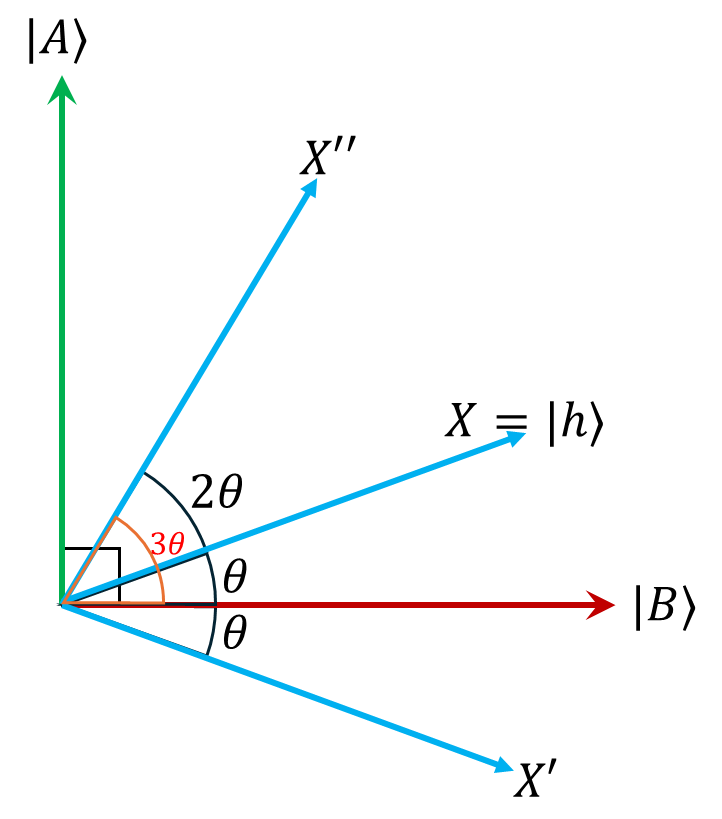
\includegraphics[width=0.5\linewidth]{Images/grover.png}
    \caption{Geometric Visualization}
    \label{fig:geometry}
\end{figure}
In the figure \ref{fig:geometry} it can be clearly seen that the$\ket{A}$ and $\ket{B}$ are orthogonal. Say $X=\ket{h}$ makes an angle $\theta$ with $\ket{B}$ (Note that for the purpose of easier imagination as said in the case where $a<<b$, (say $a=1, b=N-1$) which is mostly the case, i.e. when the number of good strings to be searched for is much less than the bad strings, the component of $\ket{h}$ on $\ket{A}$ ($=\frac{\sqrt{a}}{\sqrt{N}}$) will be much less than the component of $\ket{B}$ on $\ket{h}$ ($=\frac{\sqrt{b}}{\sqrt{N}}$) since $a<<b$. Thus, as shown in the figure \ref{fig:geometry}, $\ket{h}$ is much closer to $\ket{B}$ than $\ket{A}$.) 

Note that it is easy to create the state $\ket{h}$ since it is simply an equal superposition of all the states. Thus can be created by applying $H^{\otimes n}$ to $\ket{0^n}$. From figure \ref{fig:geometry} we are required to make a series of rotations/unitary transformations such that eventually $\ket{h}$ gets closer to $\ket{A}$ (or becomes $\ket{A}$), thus achieving the purpose of finding the superposition of strings $x \in \{0,1\}^n$ whose input to the function yields output 1. Then, upon measurement of this state we get one of the required strings whose input to the function yields output 1.

The Unitary transformations (recall that they are simply rotations or reflections in the complex Plane i.e. Hilbert Space) required to perform this are a series of reflections as follows (Starting with $\ket{X}=\ket{h}$):
\begin{enumerate}
    \item Reflect $X$ about $\ket{B}$ which as shown in the figure \ref{fig:geometry} becomes $\ket{X'}$. Say this is denoted by the Unitary matrix $R_{\ket{B}}$. Thus, $\ket{X'}=R_{\ket{B}}\ket{X}$
    \item Now reflect $\ket{X'}$ about $\ket{h}$ which as shown in the figure \ref{fig:geometry} becomes $\ket{X''}$. Say this is denoted by the Unitary matrix $R_{\ket{h}}$. Thus, $\ket{X''}=R_{\ket{h}}\ket{X'}$
\end{enumerate}
After each iteration we put $\ket{X}=\ket{X''}$ and repeat the above two steps.
Thus, the angle of $\ket{X''}$ with $\ket{B}$ is $3\theta$ after doing this reflections for the first time.
Hence, the $\ket{X''}$ obtained in the second step is now clearly closer to $\ket{A}$. Thus, performing the above steps repeatedly will bring the $\ket{X}$ closer and closer to $\ket{A}$ with each iteration as it moves farther and farther from $\ket{B}$. Once the state $\ket{X''}$ is close enough to $\ket{A}$, measuring the state will result in the required search string with a very high probability.
Thus, till now what we have done is the following:
\[
\ket{0^n}\xrightarrow{H^{\otimes n}} \ket{h}
\]
Then we repeat the following unitary transformation a finite number of times ($\mathcal{O}(\sqrt{N})$ times) starting with $\ket{X}=\ket{h}$
\[
\ket{X} \xrightarrow{R_{\ket{B}}} \ket{X'} \xrightarrow{R_{\ket{X}}} \ket{X''}
\]
Then, finally we make a measurement on $\ket{X''}$ (since it gets very close to A as shown above) and the result of that measurement is one the strings whose input to the function yields output 1. Thus, the required algorithm. This is the idea behind the Grover's algorithm.
It would suffice if we could find the two unitary transformation matrices corresponding to the reflections and show that it does perform the task of reflection about $\ket{B}$ and reflection about $\ket{X}$ respectively and along with that we are required to find the optimal number of times to repeat the process. All of this is answered in the next section.

\subsection{Algorithm}
\subsubsection{Reflection about $\ket{B}$} 
Recall that $\ket{h}$ can be written as linear superposition of the basis $\ket{A}$ and $\ket{B}$ as follows (where both $\ket{A}$ and $\ket{B}$ are orthogonal):
\[
\ket{h}=\frac{\sqrt{a}}{\sqrt{N}}\ket{A}+\frac{\sqrt{b}}{\sqrt{N}}\ket{B}
\]
In order to reflect $\ket{h}$ about $\ket{B}$, see figure \ref{fig:geometry}, we are required to reverse the component of projection of $\ket{h}$ on $\ket{A}$. Thus, the reflected vector should have the following linear superposition:
\[
\ket{X'}=-\frac{\sqrt{a}}{\sqrt{N}}\ket{A}+\frac{\sqrt{b}}{\sqrt{N}}\ket{B}
\]
In other words, all we need to do is flip the phase of the component in the direction of $\ket{A}$. For a general $\ket{X}$  which arises in some intermediate step of the iteration, (which will be a linear superposition of $\ket{A}$ and $\ket{B}$) we are required to reverse the phase on the components in the direction of $\ket{A}$ keeping the components in the direction of $\ket{B}$ unchanged. In order to achieve this, we use \textbf{Phase Query Gate}. The idea is we apply the oracle $U_f$ with the oracle qubit in the state $(\ket{0}-\ket{1})/\sqrt{2}$, just as was done in the Deutsch-Josza algorithm. If $x$ is not a solution to the search problem, applying the oracle to the state $\ket{x}(\ket{0}-\ket{1})/\sqrt{2}$ does not change the state. On the other hand, if $x$ is a solution to the search problem, then $\ket{0}$ and $\ket{1}$ are interchanged by the action of the oracle, giving a final state $-\ket{x}(\ket{0}-\ket{1})/\sqrt{2}$. The action of the oracle is thus,
\[
\ket{x}\left(\frac{\ket{0}-\ket{1}}{\sqrt{2}}\right) \xrightarrow{U_f} (-1)^{f(x)} \left(\frac{\ket{0}-\ket{1}}{\sqrt{2}}\right)
\]
Notice that the state of the oracle qubit is not changed. It turns out that this remains $(\ket{0}-\ket{1})/\sqrt{2}$ throughout the quantum search algorithm, and therefore be omitted from further discussion of the algorithm, simplifying our description. With this convention, consider the following unitary transformation on n qubits:
\[
Z_f\ket{x}=(-1)^{f(x)}\ket{x}
\]
This is also called a \textit{phase kickback}. We say that the oracle marks the solutions to the search problem, by shifting the phase of the solution. For an $N$ item search problem with $M$ solutions, it turns out that we need only apply this search oracle $\mathcal{O}(\sqrt{N/M})$ times in order to obtain a solution, on a quantum computer. This transformation would take in the superposition state and reverse the phase of only those components which are in $\ket{A}$ (i.e. whose $f(x)=1$) using linearity property of distributive action of a matrix on sum of vectors (superposition state). This discussion of the oracle without describing how it works in practice is rather abstract, and perhaps even puzzling. It seems as though the oracle already knows the answer to the search problem; what possible use could it be to have a quantum search algorithm based upon such oracle consultations?! The answer is that there is a distinction between knowing the solution to a search problem, and being able to recognize the solution; the crucial point is that it is possible to do the latter without necessarily being able to do the former. 

\begin{importantnote}
A simple example to illustrate this is the problem of factoring. Suppose we have been given a large number, $m$, and told that it is a product of two primes, $p$ and $q$ - the same sort of situation arises in trying to break the RSA public key cryptosystem. To determine $p$ and $q$, the obvious method on a classical computer is to search all numbers from $2$ through $m^{1/2}$ for the smaller of the two prime factors. That is, we successively do a trial division of $m$ by each number in the range $2$ to $m^{1/2}$, until we find the smaller prime factor. The other prime factor can be found by dividing $m$ by the smaller prime. Obviously, this search-based method requires roughly $m^{1/2}$ trial divisions to find a factor on a classical computer. 

The quantum search algorithm can be used to speed up this process. By definition, the action of the oracle upon input of the state $\ket{x}$ is to divide $m$ by $x$, and check if the division is exact, flipping the oracle qubit if this is so. Applying the quantum search algorithm with this oracle yields the smaller o the two prime factors with high probability. But to make this algorithm work, we need to construct an efficient circuit implementing the oracle. How to do this? We begin by defining the function $f(x)\equiv 1$ if $x$ divides $m$, and $f(x)=0$ otherwise, $f(x)$ tells us whether the trial division is successful or not. using the techniques of reversible computation, construct a reversible circuit which takes $(x,q)$ - representing an input register initially set to $x$ and a one bit output register initially set to $q$ - to $(x,q\oplus f(x))$, by modifying the usual (irreversible) classical circuit for doing trial division. The resource cost of this reversible circuit is the same to within a factor two as the irreversible classical circuit used for trial division, and therefore we regard the two circuits as consuming essentially the same resources. Furthermore, the classical reversible circuit can be immediately translated into a quantum circuit that takes $\ket{x}\ket{q}$ to $\ket{x}\ket{q \oplus f(x)}$, as required of the oracle. The key point is that even without knowing the prime factors of $m$, we can explicitly construct an oracle which recognizes a solution to the search problem when it sees one. Using this oracle an the quantum search algorithm we can search the range $2$ to $m^{1/2}$ using $\mathcal{O}(m^{1/4})$ oracle consultations. That is, we need only perform the trial division roughly $m^{1/4}$ times, instead of $m^{1/2}$ times, as with the classical algorithm!

The factoring example is conceptually interesting but not practical: there are classical algorithms for factoring which work much faster than searching through all possible divisors. However, it illustrates the general way in this the quantum search algorithm may be applied: classical algorithms which reply on search based techniques may be sped up using the quantum search algorithm. The quantum search algorithm offers a genuinely useful aid in speed up the solution of \textbf{NP}-complete problems.
\end{importantnote}

We now study the corresponding circuit as shown in the figure \ref{fig:reflect_about_b} which performs this transformation.
\begin{figure}[ht]
    \centering
    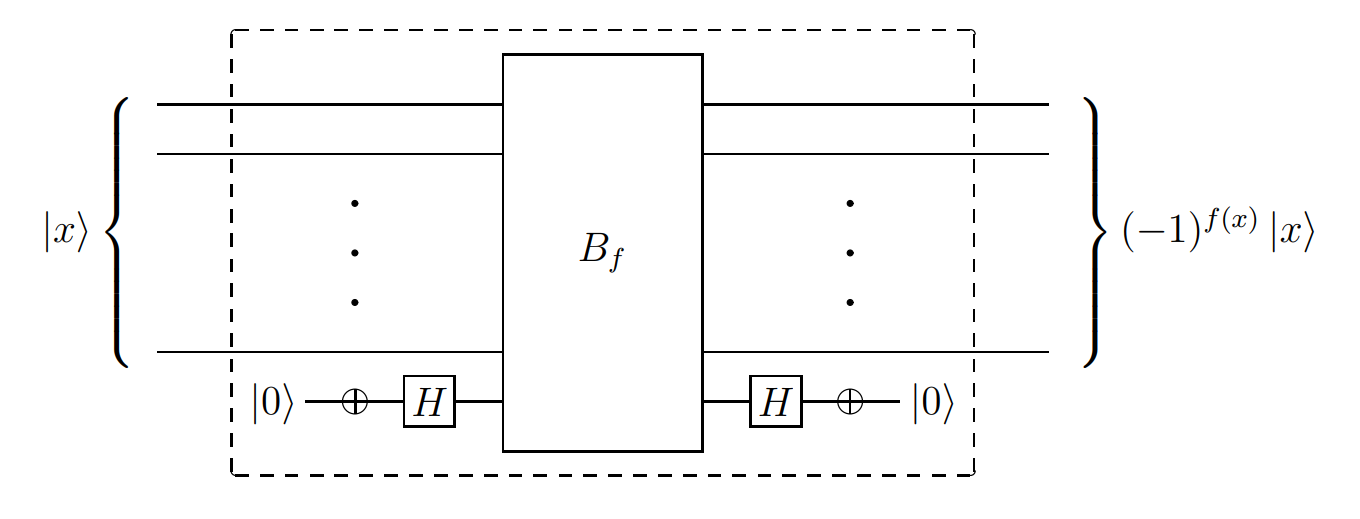
\includegraphics[width=1\linewidth]{Images/reflect_about_b.png}
    \caption{Reflection about B circuit}
    \label{fig:reflect_about_b}
\end{figure}
Here, recall that the transformation $B_f$ is the quantum implementation of the classical function $f$ i.e. $B_f\ket{x}\ket{y}=\ket{x}\ket{y\oplus f(x)}$.
We now analyse the circuit. The input to the circuit is $\ket{x}\ket{0}$. Here $\ket{0}$ is the ancilla bit. We then apply NOT-gate on the second register:
\[
\ket{x}\ket{0}\xrightarrow{I^{\otimes n}\otimes X}\ket{x}\ket{1}
\]
Then we apply a Hadamard gate on the output on the second register, thus we get,
\[
\ket{x}\ket{1}\xrightarrow{I^{\otimes n}\otimes H}\ket{x}\frac{\ket{0}-\ket{1}}{\sqrt{2}}
\]
Now we use the Oracle $B_f$ on this,
\[
B_f\ket{x}\frac{\ket{0}-\ket{1}}{\sqrt{2}}=\frac{1}{\sqrt{2}}B_f\ket{x}\ket{0}-\frac{1}{\sqrt{2}}B_f\ket{x}\ket{1}=\frac{1}{\sqrt{2}}\ket{x}\ket{0\oplus f(x)}-\frac{1}{\sqrt{2}}\ket{x}\ket{1\oplus f(x)}
\]
This can be further simplified as follows:
\[
\frac{1}{\sqrt{2}}\ket{x}\ket{f(x)}-\frac{1}{\sqrt{2}}\ket{x}\ket{\overline{f(x)}}=\ket{x}\frac{\ket{f(x)}-\ket{\overline{f(x)}}}{\sqrt{2}}=(-1)^{f(x)}\ket{x}\frac{\ket{0}-\ket{1}}{\sqrt{2}}
\]
Then we perform the uncomputation on the second register by applying a Hadamard gate and then a NOT gate as shown in the figure \ref{fig:reflect_about_b}.
\[
(-1)^{f(x)}\ket{x}\frac{\ket{0}-\ket{1}}{\sqrt{2}}\xrightarrow{I^{\otimes n}\otimes H}(-1)^{f(x)}\ket{x}\ket{1}\xrightarrow{I^{\otimes n}\otimes X}(-1)^{f(x)}\ket{x}\ket{0}
\]
Now, ignoring the ancilla bit we have thus achieved the following transformation
\[
Z_f\ket{x}=(-1)^{f(x)}\ket{x}
\]
which was the required transformation for the reflection of $\ket{X}$ over $\ket{B}$ done by reversing the phase of the components in the direction of $\ket{A}$. Note that we were required to perform one evaluation of $B_f$ implemented in $X_f$ to reflect about $\ket{B}$. Thus, what we have achieved through this Oracle as a Unitary operator can be seen from the fact that consider a $\ket{X}$ as some linear superposition of $\ket{A}$ and $\ket{B}$ (recall, $\ket{A}$ and $\ket{B}$ are orthogonal and $\ket{X}$ lies in the two-dimensional subspace spanned by $\ket{A}$ and $\ket{B}$) , say $\ket{X}=r\ket{A}+s\ket{B}$ for some $r,s$. Then upon applying the operator/Oracle $Z_f$ on this $\ket{X}$ we get,
\begin{align*}
Z_f\ket{X}&=r Z_f\ket{A}+s Z_f\ket{B}\\
&=r Z_f\frac{1}{\sqrt{a}}\sum_{x\in A}\ket{x}+s Z_f\frac{1}{\sqrt{b}}\sum_{x\in B}\ket{x}\\
&=r \frac{1}{\sqrt{a}}\sum_{x\in A}Z_f\ket{x}+s \frac{1}{\sqrt{b}}\sum_{x\in B}Z_f\ket{x}\\
&=r \frac{1}{\sqrt{a}}\sum_{x\in A}-\ket{x}+s \frac{1}{\sqrt{b}}\sum_{x\in B}\ket{x}\\
&=-r \ket{A}+s\ket{B}
\end{align*}
As can be seen that the component of $\ket{X}$ along $\ket{A}$ is reversed. Thus, we achieve the reflection about $\ket{B}$. 

Summarizing, recall that the algorithm begins with a superposition state. In order to create the superposition state $\ket{h}$, we start with $\ket{0^n}$ and apply the following hadamard transform $H^{\otimes n}$ on the state to achieve the superposition state 
\[
\ket{h}=H^{\otimes n}\ket{0^n}=\frac{1}{\sqrt{N}}\sum_{x} \ket{x}=\frac{\sqrt{a}}{\sqrt{N}}\ket{A} + \frac{\sqrt{b}}{\sqrt{N}}\ket{B}
\]
Now, since we already have the oracle $B_f$ which performs the following operation $B_f\ket{x}\ket{y} = \ket{x}\ket{y\oplus f(x)}$, then we create another oracle $Z_F$ as follows. 
For the oracle operation to perform phase kickback, the ancilla bit is prepared in $\ket{0}$ and then acted upon by Pauli NOT $X$ gate and then a Hadamard gate $H$ and after the oracle operation $B_f$ we perform uncomputation. Thus, achieving the required operation (ignoring the ancilla bit) as $Z_f\ket{x}=(-1)^{f(x)}\ket{x}$. Recall that we have already shown how to reflect any vector in the two dimensional space using the reflection about $\ket{B}$ and thus we can start by reflection $\ket{h}$ in this two dimensional space about $\ket{B}$ and then later on repeat this step to reflect any vector about $\ket{B}$ in this two dimensional space repeatedly in order to achieve the final vector close to $\ket{A}$ (or exactly $\ket{A}$). The algorithm proper makes use of single $n$ qubit register. The internal workings of the oracle, including the possibility of it needing extra work qubits, are not important to the description of the quantum search algorithm proper.

\subsubsection{Reflection about $\ket{h}$}
For the reflection about $\ket{h}$, we use the 
Diffusion operator $D$ (assume $N=2^n$), 
which works as follows. 
First, apply $H^{\otimes n}$, which maps 
$\ket{h}\rightarrow \ket{00\ldots 0}$. 
then reflect around $\ket{00\ldots 0}$ this 
is accomplished by the circuit $U_g$, where $g$ 
is a function such that $g(00\ldots 0)=0$ and $g(x)=1$ 
for $x \neq 00\ldots 0$. Finally, apply $H^{\otimes n}$ 
to return to the original basis. (Note that this is simply 
a reflection around the zero vector in the Hadamard basis). 
This is the general idea of Reflection about $\ket{h}$.
In order to understand this operation better we get into 
the details as follows.
Consider an operator $Z_0$ as follows:
\[
Z_0=I-2\ket{0^n}\bra{0^n}
\]
Thus,
\[
D=H^{\otimes n}Z_0H^{\otimes n}=H^{\otimes n}(I-2\ket{0^n}\bra{0^n})H^{\otimes n}=I-2\ket{h}\bra{h}
\]
This is also the same as having a phase query gate $Z_{OR}$ ($=-Z_0$) for the n-bit OR function:
\[
OR(x)=\begin{cases}
    0, \quad x=0^n \\ 1, \quad x\neq0^n
\end{cases}
\]
for all $x \in \{0,1\}^n$.
\[
Z_{OR}(x)=\begin{cases}
    \ket{x} \quad x=0^n \\
    -\ket{x} \quad x\neq0^n
\end{cases}
\]
for all $x \in \{0,1\}^n$. Note that $Z_{OR}=-Z_0=2\ket{0^n}\bra{0^n}-I$. Note that this does not depend on function $f$ and thus requires no queries. To implement this on a quantum circuit we convert the classical implementation of a n-bit OR boolean circuit. To perform the conditional phase shift operation $2\ket{0^n}\bra{0^n}-I$, we can implement the following circuit up to an unimportant global phase factor \ref{fig:genformcondp}.
\begin{figure}[ht]
    \centering
    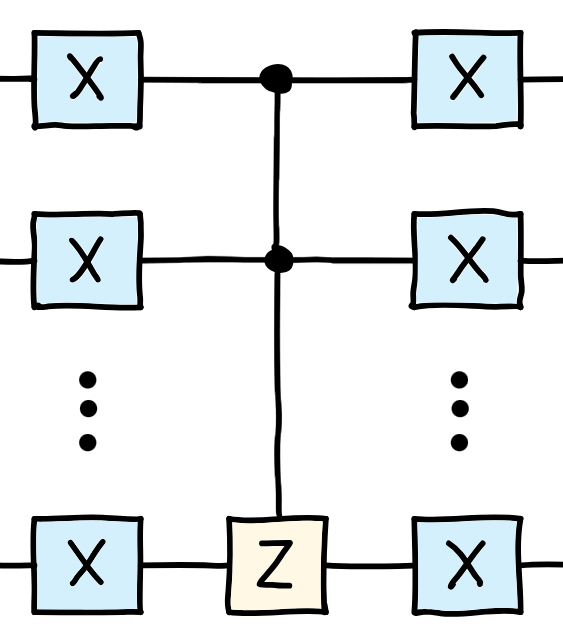
\includegraphics[width=0.5\linewidth]{Images/grov_condphase.png}
    \caption{General form of the operator $I-2\ket{0^n}\bra{0^n}$}
    \label{fig:genformcondp}
\end{figure}
Note that in this circuit the output on the input of $\ket{0^n}$ is $-\ket{0^n}$ and $\ket{x}$ where $x\neq 0^n$ is $\ket{x}$ which is opposite e of what we wanted. Thus, the given circuit in figure \ref{fig:genformcondp} implements the $-(2\ket{0^n}\bra{0^n}-I)=I-2\ket{0^n}\bra{0^n}$. But since this only affects the global phase factor and just negates the amplitudes, it does not change the probabilities. Also, we implement this operation $k$ times, in case if $k$ is even, the minus sign will vanish. In the case when $k$ is odd and there will be a minus sign, still, the resulting state would just have negative amplitudes but sine upon measurement the probabilities would not be affected and remain the same and also the result remains the same as global phase factor does not make any difference to the measurement. Thus, the complete conditional phase shift operator is as in figure \ref{fig:cond_phase}:
\begin{figure}[ht]
    \centering
    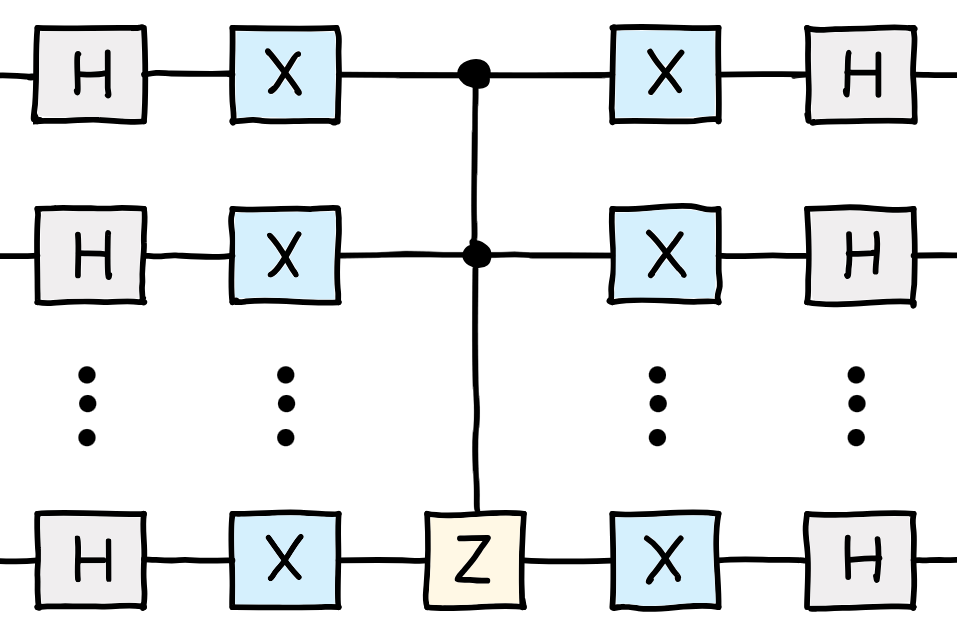
\includegraphics[width=0.5\linewidth]{Images/condphaseshift.png}
    \caption{General conditional phase shift operator implementation $I-2\ket{h}\bra{h}$}
    \label{fig:cond_phase}
\end{figure}
We now make the following propositions:
\begin{proposition}
    The Diffusion operator D has two properties:
    \begin{enumerate}
        \item It is Unitary and can be efficiently realised.
        \item It can be seen as an "inversion about the mean".
    \end{enumerate}
\end{proposition}
\begin{proof}
    \begin{enumerate}
        \item To prove that D is unitary it suffices to prove that $H^{\otimes n}$ and $Z_0$ is Unitary. Clearly, $H^{\otimes n}$ is unitary since it is a Hadamard Gate tensored product n times. Now for proving that $Z_0$ is unitary. We do as follows:
        \begin{align*}
        Z^{\dagger}_0&=(I-2\ket{0^n}\bra{0^n})^{\dagger}\\
        &=I^{\dagger}-2(\ket{0^n}\bra{0^n}^{\dagger}\\
        &=I-2\ket{0^n}\bra{0^n}=Z_0\\
        \end{align*}
        Thus, $Z_0$ is Hermitian. Now doing $Z^{\dagger}_0Z_0$, we get,
        \begin{align*}
        Z^{\dagger}Z_0=Z_0Z^{\dagger}_0&=(I-2\ket{0^n}\bra{0^n})(I-2\ket{0^n}\bra{0^n})\\
        &=I-2\ket{0^n}\bra{0^n}-2\ket{0^n}\bra{0^n}+4\ket{0^n}\bra{0^n}\\
        &=I
        \end{align*}
        Thus, $Z_0$ is Unitary. Hence $D=H^{\otimes n}Z_0H^{\otimes n}$ is a product of Unitary matrices and hence itself is a Unitary Matrix. Observe that D is expressed as the product of three Unitary matrices (two hadamard Matrices separated by a conditional phase shift matrix). Therefore, D is also Unitary. regarding the implementation, both the Hadamard and the conditional phase shift transforms can be efficiently realized within $\mathcal{O}(n)$ gates. The Hadamard transform require $\mathcal{O}(\log N)$ operations each. The conditional phase shift may be implemented using $\mathcal{O}(n)$ gates. The cost of the oracle call depends upon the specific application.
        \item Consider $D$ operating on a vector $\ket{\alpha}$ to generate another vector $\ket{\beta}$.
        \[
        D\begin{bmatrix}\alpha_1 \\ \alpha_2 \\ \vdots \\ \alpha_i \\ \vdots \\\alpha_N \end{bmatrix} = \begin{bmatrix} \beta_1\\ \beta_2 \\ \vdots \\\beta_i \\ \vdots \\ \beta_N \end{bmatrix}
        \]
        Let $\mu=\frac{1}{N}\sum_j\alpha_j$ be the mean amplitude, then the expression $2\mu-\alpha_i$ describes a reflection of $\alpha_i$ about mean. This might be easier to see by writing it as $\mu + (\mu -\alpha_i)$. In order to realise that the diffusion operator does perform this task, let us write $D$ in matrix form ($N=2^n$):
        \begin{align*}
        D&=I-2\ket{h}\bra{h}\\
        &=\begin{bmatrix} 1 & 0 & \ldots & 0 & 0 \\0 & 1 & \ldots & 0 & 0 \\ \vdots & \vdots &  \ddots & \vdots &\vdots \\0 & 0 & \ldots & 1 & 0 \\ 0 & 0 & \ldots & 0 & 1  \end{bmatrix} - \frac{2}{N}\begin{bmatrix} 1 & 1 & \ldots & 1 & 1 \\ 1 & 1 & \ldots & 1 & 1 \\\vdots & \vdots & \ddots & \vdots & \vdots \\ 1 & 1 & \ldots & 1 & 1 \\1 & 1 & \ldots & 1 & 1 \end{bmatrix} \\
        D&=\begin{bmatrix} 1 - \frac{2}{N}& -\frac{2}{N} & \ldots & -\frac{2}{N} & -\frac{2}{N} \\-\frac{2}{N} & 1-\frac{2}{N} & \ldots & -\frac{2}{N} & -\frac{2}{N} \\ \vdots & \vdots &  \ddots & \vdots &\vdots \\-\frac{2}{N} & -\frac{2}{N} & \ldots & 1-\frac{2}{N} & -\frac{2}{N} \\ -\frac{2}{N} & -\frac{2}{N} & \ldots & -\frac{2}{N} & 1-\frac{2}{N}  \end{bmatrix}
        \end{align*}
        Thus, the amplitude of $\beta_i=-\frac{2}{N}\sum_j\alpha_j+\alpha_i=-2\mu+\alpha_i$ can be considered an ``inversion about the mean" with respect to $\alpha_i$.
    \end{enumerate}
\end{proof}
\begin{example}
Show that the operation $(2\ket{\psi}\bra{\psi}-I)$ applied to a general state $\sum_k \alpha_k\ket{k}$ produces
\[
\sum_k (-\alpha_k+2\langle \alpha \rangle)\ket{k}
\]
where $\braket{\alpha} \equiv \sum_k \alpha_k/N$ is the mean value of the $\alpha_k$. For this reason, $(2\ket{\psi}\bra{\psi}-I)$ is sometimes referred to as the inversion about mean operation.

Recall that $\ket{\psi}=\frac{1}{\sqrt{N}} \sum_{x=0}^{N-1}\ket{x}$. Thus, $\ket{\psi}\bra{\psi} = \frac{1}{N}\sum_{x=0}^{N-1} \sum_{y=0}^{N-1} \ket{x}\bra{y}$. Let us apply the operation as follows:
\begin{align*}
(2\ket{\psi}\bra{\psi}-I)\sum_k \alpha_k\ket{k}&=\left(2\frac{1}{N}\sum_{x=0}^{N-1} \sum_{y=0}^{N-1} \ket{x}\bra{y} \sum_{k} \alpha_k\ket{k}-\sum_k\alpha_k\ket{k}\right)\\
&=2\frac{1}{N}\sum_k \sum_{x=0}^{N-1}\sum_{y=0}^{N-1} \alpha_k \ket{x}\bra{y}\ket{k} -\sum_k \alpha_k \ket{k}\\
&=2\frac{1}{N}\sum_k \sum_{x=0}^{N-1}\sum_{y=0}^{N-1} \alpha_k \ket{x}\delta_{y,k} -\sum_k \alpha_k \ket{k}\\
&=2\frac{1}{N}\sum_k \sum_{x=0}^{N-1} \alpha_k\ket{x} -\sum_k\alpha_k\ket{k}\\
&=2\sum_{x=0}^{N-1}\sum_k \frac{\alpha_k}{N}\ket{x} - \sum_k\alpha_k\ket{k}\\
&=2\sum_{x=0}^{N-1} \langle \alpha \rangle \ket{x}-\sum_k \alpha_k \ket{k}\\ 
&=2\langle \alpha\rangle \sum_{x=0}^{N-1} \ket{x} - \sum_{k=0}^{N-1} \alpha_k \ket{k}\\
&=2\langle \alpha \rangle \sum_{k=0}^{N-1} \ket{k} - \sum_{k=0}^{N-1} \alpha_k\ket{k}\\
&=\sum_{k=0}^{N-1} \left(2\langle \alpha \rangle - \alpha_k \right) \ket{k}\\
&=\sum_k (-\alpha_k +2\langle \alpha \rangle)\ket{k}
\end{align*}
\end{example}
Now, in order to understand how we achieve the reflection about $\ket{h}$, let us understand that the operator $D=I-2\ket{h}\bra{h}$ is a reflection operator about a hyperplane orthogonal to $\ket{h}$. Consider the vector $\ket{X'}$. Now we can write $\ket{X'}$ as a linear superposition of components along $\ket{h}$ and components orthogonal to $\ket{h}$ which is denoted by $\ket{h^{\perp}}$ ( we can do this because recall that $\ket{X'}$ and $\ket{h}$ both lie in the two-dimensional subspace spanned by the orthogonal basis $\ket{A}$ and $\ket{B}$. Thus, when we say component orthogonal to $\ket{h}$, we mean that $\ket{h^{\perp}}$ which lies in this two-dimensional subspace, since, the component of $\ket{X'}$ which is orthogonal to $\ket{h}$ will obviously lie in the plane spanned by $\ket{A}$ and $\ket{B}$). Thus, $\ket{X'}=p\ket{h}+q\ket{h^{\perp}}$ for some $p,q$. Now we apply the operator $D$ on $\ket{X'}$, we get,
\begin{align*}
D\ket{X'}&=pD\ket{h}+qD\ket{h^{\perp}}\\
&=p(I-2\ket{h}\bra{h})\ket{h}+q(I-2\ket{h}\bra{h})\ket{h^{\perp}}\\
&=p(\ket{h}-2\ket{h}\braket{h|h})+q(\ket{h^{\perp}}-2\ket{h}\braket{h|h^{\perp}}\\
&=p\ket{h}-2p\ket{h}+q\ket{h^{\perp}}\\
&=-p\ket{h}+q\ket{h^{\perp}}\\
\end{align*}
Thus, the component along $\ket{h}$ is reversed while the component along the hyperplane orthogonal to $\ket{h}$ (i.e. along $\ket{h^{\perp}}$ is preserved. Hence, it's a reflection of $\ket{X'}$ about a plane orthogonal to $\ket{h}$. Now, we simply reverse the sign i.e. use $-D$ as operator. Thus, we get,
\[
-D\ket{X'}=p\ket{h}-q\ket{h^{\perp}}
\]
which preserves the component along $\ket{h}$ and reverses the component along the plane orthogonal to $\ket{h}$ (i.e. along $\ket{h^{\perp}}$). Hence, this operation is a reflection of $\ket{X'}$ about $\ket{h}$. Thus, the operator $-D$ is the required unitary transformation operator which performs the required reflection of $\ket{X'}$ operation about $\ket{h}$.

\begin{example}
    Show that unitary operator corresponding to the phase shift in the Grover iteration is $2\ket{0}\bra{0}-I$.

    We are interested in performing a conditional phase shift on the computer, with every computational basis except $\ket{0}$ receiving a phase shift of $-1$. Let $\ket{x}$ be any $n$-qubit computational basis. Then, we have,
    \[
    2\ket{0}\braket{0|x} - \ket{x}
    \]
    Say $\ket{x}=\ket{0^n}=\ket{0}$, then in that case we would have,
    \[
    2\ket{0}\braket{0|0} - \ket{0}=2\ket{0}-\ket{0}=\ket{0}
    \]
    For any other $x$ i.e. $\ket{x}\neq \ket{0^n}$, we get,
    \[
    2\ket{0}\braket{0|x} - \ket{x} = -\ket{x}
    \]
   since, $\braket{0|x}=0$ for $\ket{x}\neq \ket{0^n}=\ket{0}$. Hence, the unitary operator corresponding to the phase shift in the grover iteration is $2\ket{0}\bra{0}-I$.
\end{example}

\subsubsection{Grover's Rotation Operator}
 The quantum search algorithm then consists of repeated application of a quantum subroutine, known as the Grover iteration or Grover operator, which we denote $G$. The Grover iteration may be broken into four steps:
\begin{enumerate}
    \item Apply the oracle $Z_f$.
    \item Apply the Hadamard transform $H^{\otimes n}$.
    \item Perform a conditional phase shift on the computer, with every computational basis state except $\ket{0}$ receiving a phase shift of $-1$.
    \[
    \ket{x}\rightarrow -(-1)^{\delta_{x,0}} \ket{x}
    \]
    \item Apply the Hadamard transform $H^{\otimes n}$.
\end{enumerate}
We have seen that using unitary operator/matrix $Z_f$ (as an oracle) we can perform the required reflection transformation about $\ket{B}$ and using $-D$ operator/matrix we can perform the required reflection transformation about $\ket{h}$. Now, let us combine the two operations into one and define the Grover's Rotation operator as follows:
\[
G=-DZ_f=-H^{\otimes n}Z_0H^{\otimes n}Z_f
\]
\begin{example}
    Show that in the $\ket{A}$, $\ket{B}$ basis, we may write the Grover iteration as 
    \[
    G=\begin{bmatrix} \cos \theta & -\sin \theta \\ \sin \theta & \cos \theta \end{bmatrix}
    \]
\end{example}
We are now interested in the action of $G$ on elements in the two-dimensional subspace spanned by $\{\ket{A},\ket{B}\}$. The action of any matrix on any element in the subspace can be determined by examining its effect on the basis vectors of the subspace. Thus, in order to determine the action of Grover's operator $G$, it is sufficient to examine its effects on the basis vectors $\ket{A}$ and $\ket{B}$ of the two-dimensional subspace. Thus, the action of $G$ on $\ket{A}$ is given as follows:
\begin{align*}
    G\ket{A}&=-H^{\otimes n}Z_0H^{\otimes n}Z_f\ket{A} \\
    &=(I-2\ket{h}\bra{h})(-Z_f)\ket{A}\\
    &=(I-2\ket{h}\bra{h})(-Z_f)\frac{1}{\sqrt{a}}\sum_{x \in A}\ket{x}\\
    &=(I-2\ket{h}\bra{h})\frac{1}{\sqrt{a}}\sum_{x \in A}-Z_f\ket{x}\\
    &=(I-2\ket{h}\bra{h})\frac{1}{\sqrt{a}}\sum_{x \in A}\ket{x}\\
    &=(I-2\ket{h}\bra{h})\ket{A}\\
    &=\ket{A}-2\ket{h}\braket{h|A}\\
\end{align*}
Upon Substituting the value of $\ket{h}=\sqrt{\frac{a} {N}}\ket{A}+\sqrt{\frac{b}{N}}\ket{B}$, and simplifying we get,
\begin{align*}
    &=\ket{A}-2\left(\sqrt{\frac{a} {N}}\ket{A}+\sqrt{\frac{b}{N}}\ket{B}\right)\left(\sqrt{\frac{a} {N}}\braket{A|A}+\sqrt{\frac{b}{N}}\braket{B|A}\right)\\
    &=\ket{A}-2\sqrt{\frac{a}{N}}\left(\sqrt{\frac{a} {N}}\ket{A}+\sqrt{\frac{b}{N}}\ket{B}\right)\\
    &=\left(1-\frac{2a}{N}\right)\ket{A}-\frac{2\sqrt{ab}}{N}\ket{B}\\
\end{align*}
Note that action of $G\ket{A}$ results in a vector in the same two-dimensional subspace spanned by $\ket{A}$ and $\ket{B}$.
and similarly action of operator $G$ on $\ket{B}$ is as follows:
\begin{align*}
    G\ket{B}&=-H^{\otimes n}Z_0H^{\otimes n}Z_f\ket{B}\\
    &=-(I-2\ket{h}\bra{h})\ket{B}\\
    &=-(\ket{B}-2\ket{h}\braket{h|B})\\
    &=-\ket{B}+2\sqrt{\frac{b}{N}}\left(\sqrt{\frac{a}{N}}\ket{A}+\sqrt{\frac{b}{N}}\ket{B}\right)\\
    &=\frac{2\sqrt{ab}}{N}\ket{A}-\left(1-\frac{2b}{N}\right)\ket{B}
\end{align*}
which is also a vector in the two-dimensional subspace spanned by $\ket{A}$ and $\ket{B}$. Thus, action of $G$ on some $\ket{X}$ in the two dimensional space spanned by $\ket{A}$ and $\ket{B}$ (say $\ket{X}=\alpha\ket{A}+\beta\ket{B}$) is $G\ket{X}=\alpha G\ket{A}+\beta G\ket{B}$. From the above results, we an see that $\ket{X}$ after applying $G$ remains in the subspace spanned by $\ket{A}$ and $\ket{B}$ with real coefficients. Let us represent the action of G on the subspace spanned by $\{\ket{A},\ket{B}\}$ as a matrix in $\ket{B},\ket{A}$ basis (both input and output basis) will be as follows:
\[
M=\begin{bmatrix} -\left(1-\dfrac{2b}{N}\right) & -\dfrac{2\sqrt{ab}}{N} \\ \dfrac{2\sqrt{ab}}{N} & \left(1-\dfrac{2a}{N}\right) \end{bmatrix} = \begin{bmatrix} \dfrac{b-a}{N} & -\dfrac{2\sqrt{ab}}{N} \\ \dfrac{2\sqrt{ab}}{N} & \dfrac{b-a}{N} \end{bmatrix}
\]
using $a+b=N$. Also, here $\ket{B}$ is the first column and $\ket{A}$ is the second column for the basis of the matrix. Notice that
\[
\begin{bmatrix} \sqrt{\dfrac{b}{N}} & -\sqrt{\dfrac{a}{N}} \\ \sqrt{\dfrac{a}{N}} & \sqrt{\dfrac{b}{N}} \end{bmatrix}^2=\begin{bmatrix} \dfrac{b-a}{N} & -\dfrac{2\sqrt{ab}}{N} \\ \dfrac{2\sqrt{ab}}{N} & \dfrac{b-a}{N} \end{bmatrix}=M
\]
Thus, M is a rotation matrix. Now, for $\theta \in (0,\pi/2)$ is the angle that satisfies
\[
\sin \theta = \sqrt{\frac{a}{N}} \quad \text{and} \quad  \cos \theta = \sqrt{\frac{b}{N}}
\]
then
\[
R_{2\theta}=\begin{bmatrix} \cos \theta &-\sin\theta \\ \sin \theta & \cos \theta \end{bmatrix}^2=\begin{bmatrix} \sqrt{\frac{b}{N}} & -\sqrt{\frac{a}{N}} \\ \sqrt{\frac{A}{N}} & \sqrt{\frac{b}{N}} \end{bmatrix}^2=M
\]
In other words, operator $G$ causes a rotation by an angle $2\theta$  in the space spanned by $\{\ket{A},\ket{B}\}$ for
\[
\theta = \sin^{-1} \sqrt{\frac{a}{N}}
\]
Thus, this is the same as defining the Grover operator as follows:
\[
G=\begin{bmatrix} \cos\alpha & -\sin \alpha \\ \sin \alpha & \cos \alpha \end{bmatrix}
\]
where $\alpha=2\theta =2sin^{-1}\sqrt{\frac{a}{N}}$. In other words, $\sin 2\theta=2\sin \theta \cos \theta$. Substituting $\sin \theta =\sqrt{\frac{a}{N}}$ and $\cos \theta = \sqrt{1-\sin^2 \theta}=\sqrt{1-\frac{a}{N}}=\sqrt{\frac{N-a}{N}}$. Thus, we get, $\sin 2\theta = 2\frac{\sqrt{a(N-a)}}{N}$.

Now, we can write the state $\ket{h}$ as follows show in figure \ref{fig:groverfig}:
\[
\ket{h}=\sqrt{\frac{b}{N}}\ket{B}+\sqrt{\frac{a}{N}}=\cos \theta \ket{B} + \sin \theta \ket{A}
\]
\begin{figure}[ht]
    \centering
    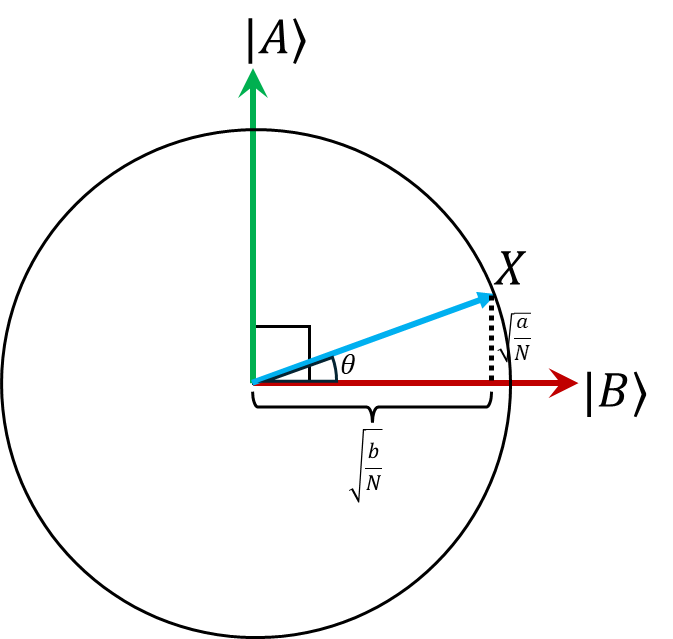
\includegraphics[width=0.6\linewidth]{Images/groverfig.png}
    \caption{Action of G}
    \label{fig:groverfig}
\end{figure}
Thus, the action of operator $G$ on $\ket{X}$ for k times (i.e. after k iterations), the state $\ket{X}$ will be,
\[
\ket{X}=\cos ((2k+1)\theta) \ket{B} + \sin((2k+1)\theta) \ket{A}
\]
We take $k=\lfloor \frac{\pi}{4}\sqrt{N}\rfloor$ for the case assuming $a=1$.
\begin{algorithm}
    \caption{Grover's Algorithm}
    \begin{algorithmic}[1]
    \State \textbf{Input:} Oracle $B_f$, number of qubits $n$
    \State \textbf{Output:} $x$ such that $f(x)) = 1$
    \State \textbf{Initialize:} $\ket{0^n}$
    \State Apply Hadamard gate to each qubit in $\ket{0^n}$, $\ket{X}=H^{\otimes n}\ket{0^n}=\frac{1}{N}\sum_{x=0}^{N-1}\ket{x}=\ket{h}$
    \State \textbf{for} $i = 1$ to $\lfloor \frac{\pi}{4}\sqrt{N} \rfloor$ \textbf{do}
    \State \hspace{1em} Apply Grover's operator $G$ on $\ket{X} \implies G\ket{X}$
    \State \hspace{1em} Set $\ket{X}=G\ket{X}$
    \State \textbf{end for}
    \State Measure the final state $\ket{X}$ in Standard Basis
    \State \textbf{return} $x$ of the measured state
    \end{algorithmic}
\end{algorithm}
Note that Measurement in the standard basis may reveal one of the candidate solutions based on the number of times we iterate the for loop. The Grover's circuit corresponding to above implementation is as shown in the figure \ref{fig:grover_circuit}.
\begin{figure}[ht]
    \centering
    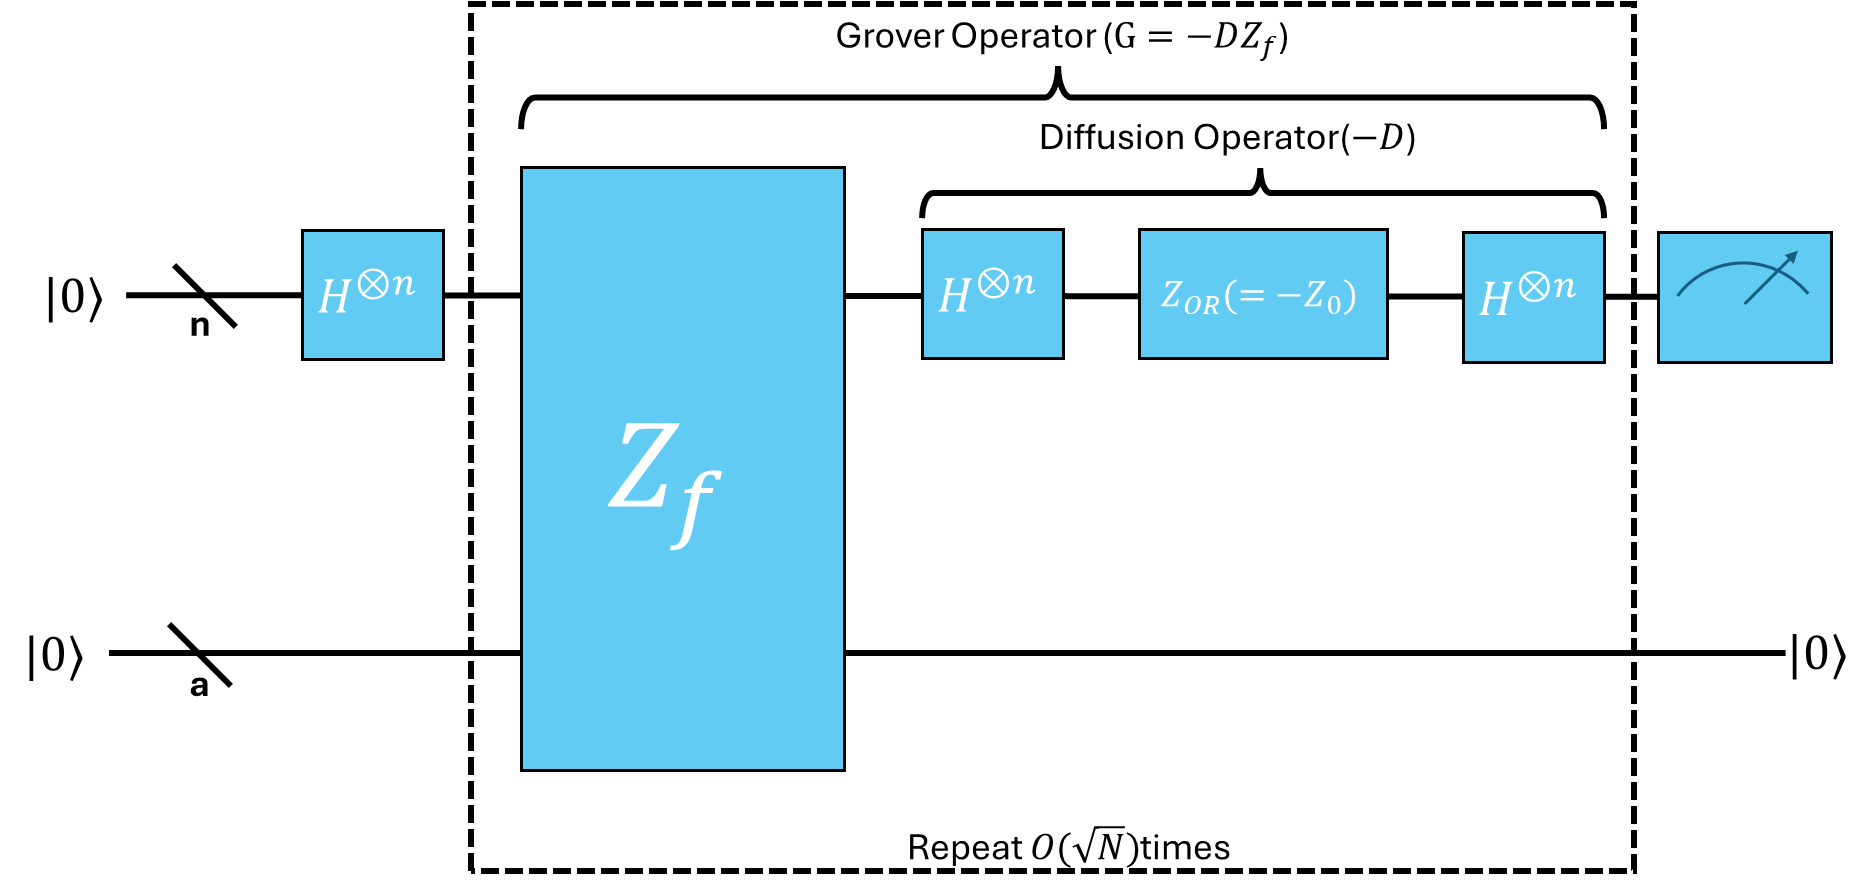
\includegraphics[width=0.9\linewidth]{Images/grovercircuit.png}
    \caption{Grover's Circuit}
    \label{fig:grover_circuit}
\end{figure}
Note that both the unitary operations $Z_f$ which is a reflection about $\ket{B}$ and reflection about $\ket{h}$ are reflection operations/transformation and hence, the determinant of those two unitary operations is $-1$. \textbf{When we compose two reflections, we obtain a rotation by twice the angle between the lines of reflection. } Consider the two-dimensional plane. There's a transformation called a reflection about a line. The way it works is: every point on one side of the line is mapped to a mirror image point on the other side of the line, as illustrated in figure \ref{fig:reflectpoints}.
\begin{figure}[ht]
    \centering
    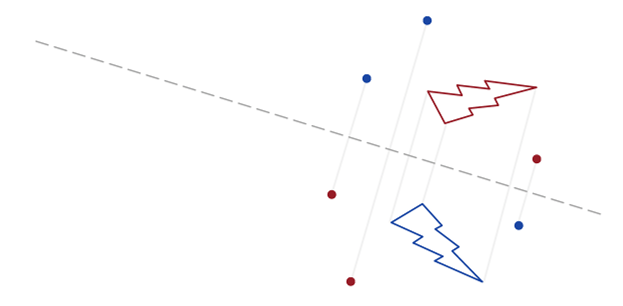
\includegraphics[width=0.75\linewidth]{Images/reflecpoitns.png}
    \caption{The reflection about the line of each red item is shown in blue}
    \label{fig:reflectpoints}
\end{figure}
Now suppose that we add a second line of reflection, with angle $\theta$ between the lines. What happens if you compose the two reflections? That is, you apply reflection 1 and then reflection 2? Let the origin be where the two lines intersect and think of each point as a vector to that point. Now, start with any such vector.
\begin{figure}[ht]
    \centering
    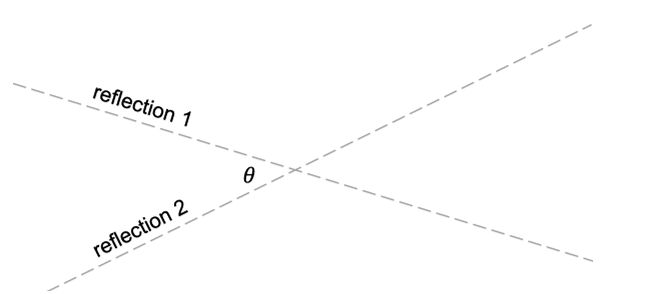
\includegraphics[width=0.75\linewidth]{Images/tworeflect.png}
    \caption{Two reflections with angle $\theta$ between them}
\end{figure}
This vector makes some angle - call it $\theta_1$ with the first line. After we perform the reflection, the reflected vector makes the same angle $\theta_1$ on the other side of the line. The reflected vector makes the some angle with the second line. Call that angle $\theta_2$. Notice that $\theta_1 + \theta_2 = \theta$. Now, if we apply the second reflection then the twice reflected vector makes an angle $\theta_2$ on the other side of the second line. So what happened to the original vector as a result of these two reflections? It has been rotated by angle $2\theta$. 
\begin{figure}[ht]
    \centering
    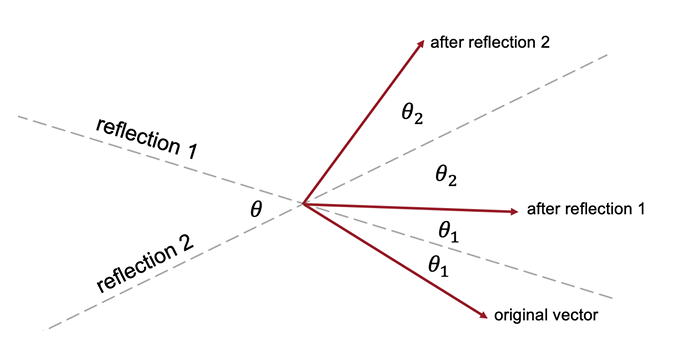
\includegraphics[width=0.75\linewidth]{Images/reflecteffect.png}
    \caption{Effect of reflection $1$ followed by a reflection $2$ on a vector}
\end{figure}
Notice that the amount of rotation depends only on $\theta$, it does not depend on what $\theta_1$ and $\theta_2$ are. 

\begin{lemma}
    For any two reflections with angle $\theta$ between them, their composition is a rotation by angle $2\theta$.
\end{lemma}
A rigorous proof can be obtained by expressing each reflection operation as a $2 \times 2$ matrix, and then multiplying the two matrices. The result will be a rotation matrix by angle $2\theta$.

Schematically, the search algorithm operates as shown in figure \ref{fig:grover_circuit}. The algorithm proper makes use of a single $n$ qubit register. The internal workings of the oracle, including the possibility of it needing extra work qubits, are not important to the description of the description of the quantum search algorithm proper. Summarizing, $G$ is a rotation in the two-dimensional space spanned by $\ket{A}$ and $\ket{B}$, rotating the space by $\theta$ radians per application of $G$. Repeated application of the Grover iteration rotates the state vector close to $\ket{A}$. When this occurs, an observation in the computational basis produces with high probability one of the outcomes superposed in $\ket{A}$, that is, a solution to the search problem.

\subsection{Example}
For example, consider the function $f:\{0,1\}^3 \rightarrow \{0,1\}$ as shown in the table \ref{tab:groverex1}.
\begin{table}[ht]
    \centering
    \begin{tabular}{|c|c|}
        \hline
        Input & Output \\
        \hline
        000 & 0 \\
        001 & 0 \\
        010 & 0 \\
        011 & 1 \\
        100 & 1 \\
        101 & 0 \\
        110 & 0 \\
        111 & 0 \\
        \hline
    \end{tabular}
    \caption{Example of Grover's Algorithm}
    \label{tab:groverex1}   
\end{table}
Thus, the set $A=\{011,100\}$ and $B=\{000,001,010,101,110,111\}$. Let the Cardinality i.e. the number of elements in the set represented as $|A|=a=2$ and $|B|=b=6$.
Here, in this example, $a=2$ and $b=6$ and $n=3$. Now, we define the vector $\ket{A}$ as:
\[
    \ket{A}=\frac{1}{\sqrt{a}}\sum_{x \in A}\ket{x}=\frac{1}{\sqrt{2}}(\ket{011}+\ket{100})
\]
Similarly, we define the vector $\ket{B}$ as:
\[
    \ket{B}=\frac{1}{\sqrt{b}}\sum_{x \in B}\ket{x}=\frac{1}{\sqrt{6}}(\ket{000}+\ket{001}+\ket{010}+\ket{101}+\ket{110}+\ket{111})
\]
Thus, it can be clearly seen that $\ket{A}$ and $\ket{B}$ are orthogonal as their inner product $\braket{A|B}=0$.\\
\textbf{STEP1: INITIALIZATION: }\\
Now, we define the vector $\ket{h}$ as an equal superposition of all the inputs by applying the Hadamard gate on  $\ket{000}$ as follows:
\begin{align*}
    H^{\otimes 3}\ket{000}&=\frac{1}{\sqrt{2^3}}\sum_{x \in \{0,1\}^3}\ket{x}\\
    &=\frac{1}{\sqrt{8}}(\ket{000}+\ket{001}+\ket{010}+\ket{011}+\ket{100}+\ket{101}+\ket{110}+\ket{111})\\
    \ket{h}&=\sqrt{\frac{2}{8}}\left(\frac{1}{\sqrt{2}}(\ket{011}+\ket{100})\right)+\sqrt{\frac{6}{8}}\left(\frac{1}{\sqrt{6}}(\ket{000}+\ket{001}+\ket{010}+\ket{101}+\ket{110}+\ket{111})\right)\\
    \ket{h}&=\sqrt{\frac{a}{N}}\ket{A}+\sqrt{\frac{b}{N}}\ket{B}
\end{align*}
\textbf{STEP2: REFLECTION ABOUT $\ket{B}$: }\\
Now we perform the reflection about $\ket{B}$ by the action of $R_{\ket{B}}=Z_f$ on the state $\ket{h}$ (recall that $Z_f\ket{x}=(-1)^{f(x)}\ket{x}$) which gives:
\begin{align*}
\ket{X'}&=Z_f\ket{h}=Z_f\frac{1}{\sqrt{8}}(\ket{000}+\ket{001}+\ket{010}+\ket{011}+\ket{100}+\ket{101}+\ket{110}+\ket{111})\\
&=\frac{1}{\sqrt{8}}(Z_f\ket{000}+Z_f\ket{001}+Z_f\ket{010}+Z_f\ket{011}+Z_f\ket{100}+Z_f\ket{101}+Z_f\ket{110}+Z_f\ket{111})\\
&=\frac{1}{\sqrt{8}}(\ket{000}+\ket{001}-\ket{010}+\ket{011}-\ket{100}+\ket{101}+\ket{110}+\ket{111})\\
&=-\sqrt{\frac{2}{8}}\left(\frac{1}{\sqrt{2}}(\ket{011}+\ket{100})\right)+\sqrt{\frac{6}{8}}\left(\frac{1}{\sqrt{6}}(\ket{000}+\ket{001}+\ket{010}+\ket{101}+\ket{110}+\ket{111})\right)\\
\ket{X'}&=-\sqrt{\frac{a}{N}}\ket{A}+\sqrt{\frac{b}{N}}\ket{B}
\end{align*}
Thus, we can clearly see that the component in the direction of $\ket{A}$ are reversed while the components in the direction of $\ket{B}$ are preserved and hence the resulting $\ket{X'}$ is a reflection about $\ket{B}$.\\
\textbf{STEP3: REFLECTION ABOUT $\ket{h}$: }\\
Now, we are required to perform a reflection of $\ket{X'}$ about $\ket{h}$ by the application of the Diffusion operator. Thus, applying $-D=-(I-2\ket{h}\bra{h})$ operator on $\ket{X'}$ gives $\ket{X''}$ as:
\begin{align*}
\ket{X''}=-D\ket{X'}&=-(I-2\ket{h}\bra{h})\ket{X'}=-(\ket{X'}-2\ket{h}\braket{h|X'})\\
&=2\braket{h|X'}\ket{h}-\ket{X'}\\
&=2\left(\sqrt{\frac{a}{N}}\bra{A}+\sqrt{\frac{b}{N}}\bra{B}\right)\left(-\sqrt{\frac{a}{N}}\ket{A}+\sqrt{\frac{b}{N}}\ket{B}\right)\ket{h}-\ket{X'}\\
&=2\left(\frac{b}{N}-\frac{a}{N}\right)\ket{h}-\ket{X'}\\
&=\frac{2(b-a)}{N} \sqrt{\frac{a}{N}} \ket{A} + \frac{2(b-a)}{N} \sqrt{\frac{b}{N}} \ket{B} + \sqrt{\frac{a}{N}}\ket{A}-\sqrt{\frac{b}{N}} \ket{B}\\
&=\left(\frac{3b-a}{N}\right)\sqrt{\frac{a}{N}}\ket{A}+\left(\frac{b-3a}{N}\right)\sqrt{\frac{b}{N}}\ket{B}\\
&=\frac{3(6)-2}{8}\sqrt{\frac{2}{8}}\ket{A}+\frac{6-3(2)}{8}\sqrt{\frac{6}{8}}\ket{B}\\
&=\frac{16}{8}\frac{1}{2}\ket{A}+0\\
&=\ket{A}\\
&=\frac{1}{\sqrt{2}}(\ket{100}+\ket{011})
\end{align*}
Initially the angle between $\ket{h}$ and $\ket{B}$ was $\braket{h|B}=\sqrt{\frac{b}{N}}=\cos \theta \implies \theta = \cos^{-1} \sqrt{\frac{6}{8}}=\frac{\pi}{6}$. After the transformation we can clearly see that the angle between $\ket{X''}$ and $\ket{B}$ is $\braket{X''|B}=0=\cos \theta \implies \theta = \cos^{-1} 0 = \frac{\pi}{2}$. Thus, the angle changed from $\frac{\pi}{6}$ to $\frac{\pi}{2}$. Thus, we can clearly see that the angle changed from $\theta$ to $3\theta$. Now, we need to repeat this reflection transformation $k=\lfloor \frac{\pi}{4}\sqrt{8}\rfloor = 2$. Thus, we need to perform this once again. But note thatwe have already arrived at $\ket{A}$ and doing this once agina will bring us farther from $\ket{A}$. This is the problem with the grover's algorithm. Since, we don't know the number of possible outcomes i.e. $a=1$ or $a \geq 1$, we assumed that $a=1$ and decided to perform the iterations based on $a=1$ which comes out as $k=\lfloor \frac{\pi}{4}\rfloor=2$. But, if we perform the operation once again then the angle between $\ket{X''}$ and $\ket{B}$ would become $5\theta=5\frac{\pi}{6} > \frac{\pi}{2}$, thus it overshoots, decreasing the probability of outcomes being from state $\ket{A}$. In order to improve over this we introduce modified grover's algorithm which states to set m=1, pick $k\in1,\ldots, m+1$ uniformly  and perform the grover's algorithm $k$ times and then perform the measurement, and stop only if we get x such that $f(x)=1$. Else, if $m<\sqrt{N}$ set $m=\lfloor (8/7)m\rfloor$, else fail.\\
\textbf{STEP4: MEASUREMENT: }\\
Thus, supposed we pick $k=1$ and then we perform the Grover's algorithm $k=1$ times, we would get the state $\ket{X''}=\ket{A}$,
\[
\ket{X''}=\ket{A}=\frac{1}{\sqrt{2}}(\ket{011}+\ket{100})
\]
thus upon performing measurements we would get the required search strings $x=\ket{100}$ and $x=\ket{011}$ with the property that $f(x)=1$ with equal probability. The Modified Grover's Algorithm is further explained in the following complexity analysis section (refer section \ref{sec:Complexity Analysis_Grover}).

\begin{example}
    \textbf{(Quantum search: a two-bit example)} Here is an example illustrating how the quantum search algorithm works on a search space of size $N=4$. The oracle, for which $f(x)=0$ for all except $x=x_0$, in which case $f(x_0)=1$, can be taken to be one of the four circuits
\begin{figure}[ht]
    \centering
    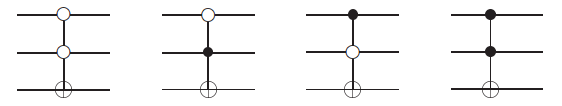
\includegraphics[width=0.75\linewidth]{Images/grov_examp.png}
\end{figure}
    corresponding to $x_0=0,1,2$ or $3$ from left to right, where the top two qubits carry the query $x$, and the bottom qubit carries the oracle's response. The quantum circuit which performs the initial Hadamard transform and a single Grover iteration $G$ is

    Initially, the top qubits are prepared in the state $\ket{0}$, and the bottom one as $\ket{1}$. The gates in the dotted box perform the conditional phase shift operation $\ket{00}\bra{00}-I$. How many times must we repeat $G$ to obtain $x_0$? Using $M=1$, we find that less than one iteration is required. It turns out that because $\theta=\pi/3$, only exactly one iteration is required to perfectly obtain, $x_0$ in this special case. In the geometric picture of figure \ref{fig:groverfig}, our initial state $\ket{\psi}=(\ket{00}+\ket{01}+\ket{10}+\ket{11})/\sqrt{2}$ is $30$ degree from $\ket{B}$, and a single rotation by $60$ degree moves $\ket{\psi}$ to $\ket{A}$. You can confirm for yourself directly, using the oracle only once. In contrast, a classical computer, or a classical circuit - trying to differentiate between the four oracles would require on average $2.25$ oracle queries!
    \begin{figure}[ht]
        \centering
        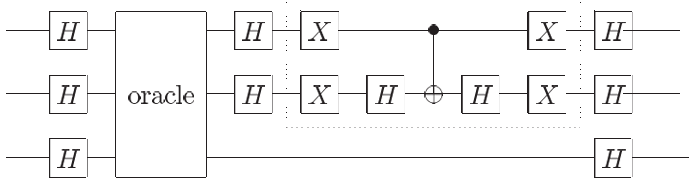
\includegraphics[width=0.75\linewidth]{Images/grover_example.png}
    \end{figure}
\end{example}
\section{Complexity Analysis}\label{sec:Complexity Analysis_Grover}Here we answer why the number of times to iterate is $\lfloor \frac{\pi}{4}\sqrt{N} \rfloor$ and thus the time complexity of the Grover's algorithm is $\mathcal{O}(\sqrt{N})$. Recall, that after k iterations of applying operator $G$ on $\ket{X}$, the state $\ket{X}$ is:
\[
\cos ((2k+1)\theta) \ket{B} + \sin ((2k+1)\theta)\ket{A}
\]
The goal is to measure some element $x \in A$, so we would like the state $\ket{X}$ to be as close to $\ket{A}$ as possible. In other words, we want the probability of measuring $\ket{A}$ to be as high as possible which consequently means that the probability of measuring $\ket{B}$ to be as low as possible. Thus, we want,
\[
\sin^2 ((2k+1)\theta) \approx 1
\]
then we require the minimum value of $k$ with which we can achieve this,
\[
(2k+1)\theta \approx \frac{\pi}{2}
\]
will suffice, so we should choose
\[
k \approx \frac{\pi}{4\theta}-\frac{1}{2}
\]
Of course k must be an integer, which is why we can only hope to approximate the quantity. Thus, putting $\theta = \sin^{-1} \sqrt{\frac{a}{N}}$, we get,
\[
k \approx \frac{\pi}{4 \sin^{-1} \sqrt{\frac{a}{N}}} - \frac{1}{2}
\]
Thus, since k must be an integer,
\[
k = \lfloor \frac{\pi}{4 \sin^{-1} \sqrt{\frac{a}{N}}} \rfloor
\]
Note that $k$ depends on angle $\theta$ which in turn depends on $a$ which is the number of solutions. Thus, the number of iterations depends on number of solutions $a$ but not on the identity of those solutions. In general, we might not know how many solutions there are so we can't pick the value of $a$ and thus, don't know the number of iterations $k$ to perform.
\subsection{Unique Search Problem}
This is the case which Lov Grover considered in his original paper in 1996 where he introduced Grover's Algorithm. Suppose for simplicity, which also turns out to be the worst case we would have $a=1$ i.e. only one unique solution string $x$ satisfying such that $f(x)=1$ and hence, for very small $\theta$, $\sin^{-1} \theta \approx \theta \implies \sin^{-1}\frac{1}{\sqrt{N}} \approx \frac{1}{\sqrt{N}}$.
\[
k \approx \frac{\pi}{4}\sqrt{N} -\frac{1}{2}
\]
\[
k \approx \frac{\pi}{4}\sqrt{N}
\]
Thus, we use $k=\lfloor \frac{\pi}{4}\sqrt{N} \rfloor$ for our algorithm. Now, recall that the operator $G$ includes the operator $Z_f$ which queries the black box (oracle) $B_f$. Thus, the number of queries needed by the algorithm is equal to the number of times we use the Grover operator which is also $k$ and thus, the queries required for the algorithm is $\mathcal{O}(\sqrt{N})$.

Note that $a=1$ represents only a special case which is coincidentally also the worst case for the searching algorithm. Thus, with the choice of $k=\lfloor \frac{\pi}{4}\sqrt{N} \rfloor$, the probability of finding the single x such that $f(x)=1$ is
\[
\sin^2 \left(\left(2\lfloor \frac{\pi}{4}\sqrt{N} \rfloor+1\right)\sin^{-1} \frac{1}{\sqrt{N}}\right)
\]
Thus, the limit of this probability is 1 as N goes to infinity, and it is at least $1/2$. This is as shown in the following table \ref{tab:Probdist}

\begin{table}[ht]
    \centering
    \begin{tabular}{c|c}
        N & Probability\\
        \hline
        2	& 0.5000000000 \\
        4	& 1.0000000000 \\
        8	& 0.9453125000 \\
        16	& 0.9613189697 \\
        32	& 0.9991823155 \\
        64	& 0.9965856808 \\
        128	& 0.9956198657 \\
        256	& 0.9999470421 \\
        512	& 0.9994480262 \\
        1024	& 0.9994612447 \\
        2048	& 0.9999968478 \\
        4096	& 0.9999453461 \\
        8192	& 0.9999157752 \\
        16384	& 0.9999997811 \\
        32768	& 0.9999868295 \\
        65536	& 0.9999882596 \\
        131072	& 0.9999992587 \\
        262144	& 0.9999978382 \\
        524288	& 0.9999997279 \\
    \end{tabular}
    \caption{Unique Search $(a=1)$: Success Probability at various $N$}
    \label{tab:Probdist}
\end{table}
So even in the worst case, repeating the algorithm some small constant number of times and evaluating $f$ at the output each time will find the unique $x$ such that $f(x)=1$ with very high probability.

Notice that these probabilities are not strictly increasing. In particular, we have an interesting anomaly when $N=4$, where we get a solution with certainty. It can be proved analytically that
\[
p(N,1)\geq 1-\dfrac{1}{N}
\]
where $p(N,1)$ is the probability of finding the required search string $x$ upon measurement. Notice that even a weak bound such as $p(N,1)\geq 1/2$ establishes the utility of Grover's algorithm. For whatever measurement outcome x we obtain from running the procedure, we can always check to see if $f(x)=1$ using a single query to $f$. And if we fail to obtain the unique string x for which $f(x)=1$ with probability at most $1/2$ by running the procedure once, then ater m independent runs of the procedure we will have failed to obtain this unique string $x$ with probability at most $2^{-m}$, That is using $\mathcal{O}(m\sqrt{N})$ queries to f, we will obtain the unique solution $x$ with probability at least $1-2^{-m}$. Using the better bound $p(N,1) \geq 1-\frac{1}{N}$ reveals that the probability to find $s \in A$ using this method is actually at least $1-N^{-m}$. Thus, as can be seen that the probabilities for the case $a=1$ approaches 1 as we increase $N$.

\subsection{Multiple Solutions}
What if $f$ has more than one satisfying input? One might be tempted to think intuitively that the ``hardest" case for the search is where there is just one satisfying input. Finding a needle in a haystack is harder if the haystack contains a single needle. So how well does the algorithm with $k\approx \frac{\pi}{4}\sqrt{N}$ iterations do when there are more satisfying inputs? Unfortunately, it's not very good. In the case when we do not know that $a=1$, the situation is more challenging.

Suppose that there are four satisfying inputs. Then $\theta \approx \frac{2}{\sqrt{N}}$. Then $\theta \approx \frac{2}{\sqrt{N}}$ (double the value in the case of one satisfying input), which causes the rotation to overshoot. The total rotation is by 180 degree instead of 90 degrees. The state starts off almost orthogonal to $\ket{A}$. Then, midway, it gets close to $\ket{A}$. And then it keeps on rotation and becomes almost orthogonal to $\ket{A}$ again.  For example, if $a=4$ but we still choose $k=\lfloor \frac{\pi}{4}\sqrt{N}\rfloor$, the probability of success is given as: 
\[
\sin^2 \left(\left(2\lfloor \frac{\pi}{4}\sqrt{N} \rfloor+1\right)\sin^{-1} \sqrt{\frac{a}{N}}\right)
\]
thus, the success probability goes to 0 in the limit of large $N$ as seen in table \ref{tab:multiple_solns}.

\begin{table}[ht]
    \centering
    \begin{tabular}{c|c}
    N & Probability \\
    \hline
        4	& 1.0000000000 \\
        8	& 0.5000000000 \\
        16	& 0.2500000000 \\
        32	& 0.0122070313 \\
        64	& 0.0203807689 \\
        128	& 0.0144530758 \\
        256	& 0.0000705058 \\
        512	& 0.0019310741 \\
        1024	& 0.0023009083 \\
        2048	& 0.0000077506 \\
        4096	& 0.0002301502 \\
        8192	& 0.0003439882 \\
        16384	& 0.0000007053 \\
        32768	& 0.0000533810 \\
        65536	& 0.0000472907 \\
        131072	& 0.0000030066 \\
        262144	& 0.0000086824 \\
        524288	& 0.0000010820 \\ 
    \end{tabular}
    \caption{Multiple Solutions: Success Probability at various N}
    \label{tab:multiple_solns}
\end{table}


This is because we are effectively rotation twice as far as we should. When there are four satisfying inputs, the ideal number of iterations is half the number for the case of one satisfying input. More generally, when there are $a$ satisfying inputs, the ideal number of iterations is $k\approx \frac{\pi}{4}\sqrt{\frac{N}{a}}$. If we know the number of satisfying inputs in advance then we can tune $k$ appropriately. Generalizing what was claimed earlier, it can be proved that 
\[
p(N,a) \geq 1 -\dfrac{a}{N}
\]
This lower bound of $1-\frac{a}{N}$ on the probability of success is slightly peculiar in that more solutions implies a worse lower bound - but under the assumption that $a$ is significantly smaller than $N$, nevertheless conclude that the probability of success is reasonably high. As before, the mere fact that $p(N,a)$ is reasonably large implies the algorithm's usefulness.
It is also the case that
\[
p(N,a) \geq \frac{a}{N}
\]
This lower bound describes the probability that a string $x \in \{0,1\}^n$ selected uniformly at random is a solution - so Grover's algorithm always does at least as well as random guessing. In fact, Grover's algorithm is random guessing when $k=0$.
As the number of elements $a$ varies, so does he angle $\theta$, which can have a significant effect on the algorithm's probability of success.
In case we know $a$ in advance and we choose the corresponding value of $k$ as 
\[
k=\lfloor \dfrac{\pi}{4\sin^{-1}\sqrt{\frac{a}{N}} }\rfloor
\]
then the probability $p(N,a)$ for finding one of the solutions upon measuring is given by
\[
p(N,a) \geq max\{1-\dfrac{a}{N},\dfrac{a}{N}\}
\]
thus, as $a/N$ goes smaller and smaller the probability approaches 1.
We now need to see how does the number of queries $k$ depend on $N$ and $a$.
\[
sin^{-1} (x) \geq x \quad \text{for every $x \in [0,1]$}
\]
\begin{align*}
    \theta &=\sin^{-1} \left(\sqrt{\frac{a}{N}}\right) \geq \sqrt{\frac{a}{N}}\\
    \implies k&\leq \dfrac{\pi}{4\theta} \leq \dfrac{\pi}{4}\sqrt{\frac{N}{a}}\\
    k&=\mathcal{O}\left(\sqrt{\frac{N}{a}}\right)
\end{align*}

\begin{algorithm}
\caption{Grover's Algorithm}
    \begin{algorithmic}[1]
        \State \textbf{Input:}(1) A black box oracle $O$ which performs the transformation $O\ket{x}\ket{q}=\ket{x}\ket{q\oplus f(x)}$, where $f(x)=0\forall 0<x<2^n$ except $x_i$ for $1\leq i\leq m$ for which $f(x_i)=1$; (2) $n+1$ qubits in the state $\ket{0}$.
        \State \textbf{Output:} One of the $x_i$
        \State \textbf{Runtime:} $\mathcal{O}(\sqrt{N/a})$ operations. Succeeds with probability $\mathcal{O}(1)$.
        \State \textbf{Procedure:}\\
        \hspace{1em}\textbf{Initial State} $\ket{0}^{\otimes n} \ket{0}$\\
        \hspace{1em} \textbf{Apply $H^{\otimes n}$ to the first $n$ qubits, and $HX$ to the last qubit.} $\rightarrow \frac{1}{\sqrt{2^n}}\sum_{x=0}^{2^n-1}\ket{x}\left( \frac{\ket{0}-\ket{1}}{\sqrt{2}}\right)$\\
        \hspace{1em} \textbf{Apply the Grover iteration $k=\lceil \frac{\pi}{4}\frac{\sqrt{2^n}}{a}\rceil$ times.}\\
        $\rightarrow [(2\ket{\psi}\bra{\psi} -I)O]^k \frac{1}{\sqrt{2^n}}\sum_{x=0}^{2^n-1}\ket{x}\left(\frac{\ket{0}-\ket{1}}{\sqrt{2}}\right)$\\
        $\approx \frac{1}{\sqrt{2^m}}\sum_{i=1}^m \ket{x_i}\left(\frac{\ket{0}-\ket{1}}{\sqrt{2}}\right)$\\
        \hspace{1em} \textbf{Measure the first $n$ qubtis}$\rightarrow x_k$ 
    \end{algorithmic}
\end{algorithm}

What happens when more than half the items are solutions to the search problem, that is $a \geq N/2$? From the expression $k=\lceil \frac{\pi}{4}\sqrt{\frac{N}{a}}\rceil$ and $\theta=\sin^{-1}\frac{\sqrt{a(N-a)}}{N}$ we see that the angle $\theta$ gets smaller as $a$ varies from $N/2$ to $N$. As a result, the number of iterations needed by the search algorithm increases with $a$, for $a\geq N/2$. Intuitively, this is a silly property for a search algorithm to have: we expect that it should become easier to find a solution to the problem as the number of solutions increases. There are at least two ways around this problem. If $a$ is known in advance to be larger than $N/2$ then we can just randomly pick up an item in the search space, and then check that it is a solution using the oracle. This approach has a success probability at least one-half, and only requires on consultation with the oracle. It has the disadvantage that we may not know the number of solutions $a$ in advance.

In the case where it isn't known whether $a\geq N/2$, another approach can be used. This approach is interesting in its own right, and has a useful application to simplify the analysis of the quantum algorithm for counting the number of solutions to the search problem. the idea is to double the number of elements in the search space by adding $N$ extra items to the search space, none of which are solutions. As a consequence, less than half the items to the search space are solutions. This is effected by adding a single qubit $\ket{q}$ to the search index, doubling the number of items to be searched to $2N$. a new augmented oracle $O'$ is constructed with marks an item only if it is a solution to the search problem and the extra bit is set to zero. The new scratch problem has only $M$ solutions out of $2N$ entries, so running the search algorithm with the new oracle $O'$ we see that at most $k=\frac{\pi}{4}\sqrt{2a/N}$ calls to $O'$ are required, and it follows that $\mathcal{O}(\sqrt{N/a})$ calls to $O$ are required to perform the search.

\begin{example}
    Show that the augmented oracle $O'$ may be constructed using one application of $O$, and elementary quantum gates, using the extra qubit $\ket{q}$.

    The following circuit can be used:
    \begin{figure}[ht]
        \centering
        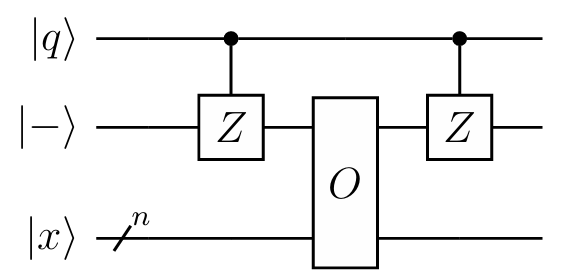
\includegraphics[width=0.75\linewidth]{Images/oracleop.png}
        \caption{Circuit for oracle $O'$}
        \label{fig:oracleop}
    \end{figure}
If $\ket{q}$ is set then on the second qubit we have $\ket{-}\rightarrow \ket{+}$, hence the oracle performs $\ket{x}\ket{+}\rightarrow \ket{x}\ket{+ \oplus f(x)}=\ket{x}\ket{+}$ i.e. no solutions are marked. If the $\ket{q}$ is not set then the oracle functions as intended i.e. marking the correct solutions. This idea is also used in Quantum Counting.
\end{example}

But suppose we're given a black box for $f$ without any information about the number of satisfying inputs that satisfy $f$. What do we do then? For any particular setting of $k$, it's conceivable that the number of satisfying inputs to $f$ is such that the total rotation after $k$ iterations is close to a multiple of 180 degrees.

In the case when the number of solutions is unknown i.e. we don't know the value of a. When we don't know the number of solutions, there are different strategies for dealing with this problem. One possibility is simply choose a random value uniformly for
\[
k\in\{1,\ldots, \lfloor \frac{\pi}{4}\sqrt{N}\rfloor\}
\]
I will roughly sketch an approach that resolves this by setting $k$ to be a random selection from the set $\{1,2,\ldots,\lceil \frac{\pi}{4}\sqrt{N}\rceil\}$ results in a success probability close to $1$. But if $k$ is set randomly then the success probability is the average value of the curve. By the symmetry of the sine curve, the area under the curve is half of the area of the box, so the success probability is $1/2$.

Now, let's consider the cases of two, three or four satisfying assignments. These cases result in larger $\theta$, and the corresponding success probability curves are as shown in figure (they are sinusoidal curves corresponding to more total rotation).

By inspection, the area under each of the curves is at least $\frac{1}{2}$. Each curve is a 90 degree rotation, for which the average is $\frac{1}{2}$, followed by another rotation less than or equal to 90 degrees, for which the average can be seen to be more than $\frac{1}{2}$.

But there are cases where the average is less than $\frac{1}{2}$. Let's look at the case of six satisfying inputs. 

There are two 90-degree rotations, followed by a rotation less than 90 degrees for which the average is less than $\frac{1}{2}$. Teh average for the whole curve can be calculated to be around $0.43$.  For larger numbers of satisfying inputs, the proportion of the domain associated with the last partial rotation becomes small enough so as the be inconsequential.

The idea is that we are giving the state vector $\ket{X}$ a random rotation. This does not make the probability of getting a solution close to 1 but the probability of finding a solution (if one exists) will be at least 40\%. We can now boost the probability of getting the correct solution exponentially by repeating this process choosing k independently each time. The chance of not finding a solution decreases exponentially in the number of time we repeat. For example to increase probability to 99\% we can run this algorithm 10 times with k chosen independently each time. The number of queries is still $\mathcal{O}(\sqrt{N})$ (or evaluations of $f$) even when we don't know the number of solutions in advance. Still operating under the assumption $a\geq 1$, the algorithm will fail to find an $x$ with $f(x)=1$ with probability at most $3/4$. Repeating some constant number of times until a "good" $x$ is found quickly decreases error. The above roughly explains why choosing $k$ randomly within the range results in a success probability that's at least $0.43$, regardless of the number of satisfying assignments. That's one way to solve the case of an unknown number of satisfying inputs to $f$.

To summarize, ewe have a quantum algorithm that makes $\mathcal{O}(\sqrt{N})$ queries and finds a satisfying assignment with constant probability. By repeating the process a constant number of times, the success probability can be made close to $1$.

There is a refined version of the search algorithm that stops early, depending on the number of satisfying inputs. The number of queries is $\mathcal{O}(\sqrt{\frac{N}{a}})$, where $a$ is the number of satisfying inputs. This refined algorithm does not have information about the value of $a$. When the algorithm is run, we don't know in advance for how long it will need to run. A somewhat better strategy is to apply the method above for successively larger values. Specifically, instead of choosing a random k in the range $1,\ldots, \lfloor \frac{\pi}{4}\sqrt{N}\rfloor$, do the following:

\begin{algorithm}
    \caption{Modified Grover's Algorithm for $a \geq 1$}
    \begin{algorithmic}[1]
    \State Set $m=1$.
    \State Choose $ k \in \{1,\ldots, m+1\}$ uniformly at random and run Grover's algorithm for this choice of $k$. If the algorithm finds an $x$ such that $f(x)=1$, then output $x$ and halt.
    \State If $m>\sqrt{N}$ then "fail". Else set $m=\lfloor (8/7)m\rfloor$ and goto step 2.
    \end{algorithmic}
\end{algorithm}
This will succeed in finding $x \in A$ with probability at least $1/4$ after $\mathcal{O}(\sqrt{\frac{N}{a}})$ queries. By repeating step 2 a constant number of times during each iteration of the loop, the error decreases exponentially. (the number $8/7$ just happens to be a number that works for the analysis, which we will not discuss. The point is that m increases exponentially, but not too fast to cause the algorithm to fail). Another choice is to use $\lfloor \frac{5}{4}k\rfloor$. The rate of increase of k must be carefully balanced; slower rates require more queries, higher rates decrease success probability. If the number of solutions is $a\geq 1$, then the number of queries (or evaluations of $f$) required is $\mathcal{O}(\sqrt{N/a})$. If there are no solutions $\mathcal{O}(\sqrt{N})$ queries are required.

\subsection{Trivial Case}
Finally we need to deal with the special cases when $a=0$ or $b=0$. Obviously if $a=0$, the output $x$ of the algorithm will never satisfy $f(x)=1$ because there are no such values of $x$. It is easy to check directly that Grover's Algorithm will output a choice of $x \in \{0,1\}^n$ that is uniformly distributed in this case. In that case, the algorithm will not find a satisfying assignment in any runs and outputs ``unsatisfiable". The situation where one of A and B is empty happens when $f$ is constant; A is empty when $f(x)=0$ for every $x \in \{0,1\}^n$, and B is empty when $f(x)=1$ for every $x\in\{0,1\}^n$. This means that
\[
Z_f\ket{h}=\pm \ket{h}
\]
and therefore
\begin{align*}
    G\ket{h}&=(2\ket{h}\bra{h}-I)Z_f\ket{h}\\
    &=\pm (2\ket{h}\bra{h}-I)\ket{h}\\
    &=\pm \ket{h}
\end{align*}
So, irrespective of the number of iterations $k$ we perform in these cases, the measurement always reveals a uniform random string $x \in \{0,1\}^n$.
Supposing that we do not know $a$, if we run Grover's Algorithm as described above and always measure a value of $x$ for which $f(x)=0$, we can reasonable conclude with high confidence that $a=0$. It is also the case when $b=0$ that Grover's Algorithm will output a uniformly distributed choice of $x$. Of course in this case $f(x)=1$ for all $x$, so the problem is trivially solved.

\section{Optimality of Grover's algorithm}
In this section we will prove that grover's algorithm is optimal in terms of the number of black-box queries that it makes. We have show that a quantum computer can search $N$ items, consulting the search oracle only $\mathcal{O}(\sqrt{N})$ times. We now prove that no quantum algorithm can perform this task using fewer than $\Omega(\sqrt{N})$ accesses to the search oracle, and thus the algorithm we have demonstrated is optimal.

\begin{theorem}
    \textbf{(optimality of grover's algorithm)} Any quantum algorithm for the search problem for functions of the form $f:\{0,1\}^n \rightarrow \{0,1\}$ that succeeds with probability at least $\frac{3}{4}$ must make $\Omega(\sqrt{2^n})$ queries.
\end{theorem}
\begin{proof}
    We make the following two simplifying assumptions.
    \begin{enumerate}
        \item Assume that the function is always queried in the phase (as occurs with Grover's algorithm). To determine $x$ we are allowed to apply an oracle $Z_f$ which gives a phase shift of $-1$ to the solution and leaves all other states invariant, $Z_f=I-2\ket{x}\bra{x}$.
        \begin{figure}[ht]
            \centering
            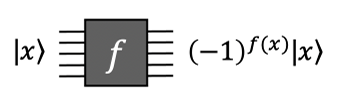
\includegraphics[width=0.5\linewidth]{Images/groveropt.png}
        \end{figure}
        \item Assume that the algorithm uses only $n$ qubits. That is, no ancilla qubits are used.
    \end{enumerate}
    For simplicity, we prove the lower bound for the case where the search problem has a single solution, $x$. The purpose of these simplifying assumptions is to reduce clutter. it is very straightforward to adjust the proof to the general case, where the function is queried in the standard way, and where the quantum algorithm is allowed to use ancilla qubits. The more general proof will be just a more cluttered-up version of the proof about to be explained. Noting of importance is being swept under the rug in this simplified proof.

    Under our assumptions, any quantum algorithm that makes $k$ queries in a circuit is of the form \ref{fig:kquery}.
    \begin{figure}[ht]
        \centering
        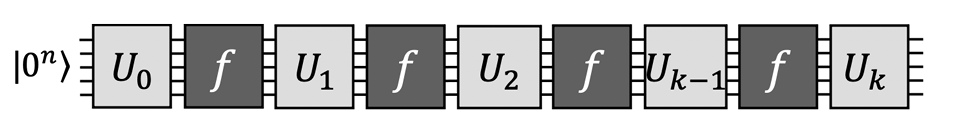
\includegraphics[width=0.75\linewidth]{Images/kquery.png}
        \caption{Form of a $k$ query quantum circuit}
        \label{fig:kquery}
    \end{figure}
    The initial state of the $n$ qubits is $\ket{0^n}$. Then an arbitrary unitary operation $U_0$ is applied, which can create any pure state (say $\ket{\psi}$) as the input to the first query. Then the second $f$-query is performed. And so on, up to the $kth$ $f-$ query, followed by an arbitrary unitary operation $U_k$. The success probability is the probability that a measurement of the final state results in a satisfying input of $f$.

    The quantum algorithm is the specification of the unitaries $U_0, U_1 ,\ldots, U_k$. The input to the algorithm is the black box for $f$, which is inserted into the $k$ query gates. The quantum output is the final state produced by the quantum circuit. The overall approach will be as follows. 
    For every $r \in \{0,1\}^n$, define $f_r$ as
    \[
    f_r (x) = \begin{cases} 1 &\text{if $x=r$}\\
    0 &\text{otherwise} \end{cases}
    \]
    We'll show that, for any algorithm that makes asymptotically fewer than $\sqrt{2^n}$ queries, it's success probability is very low for at least one $f_r$.

    Assume that we have some $k$-query algorithm, specified by $U_0,U_1,\ldots, U_k$. Suppose that we insert one of the function $f_r$ into the query gate.
\begin{figure}[ht]
    \centering
    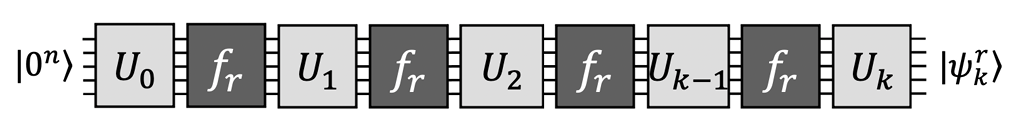
\includegraphics[width=0.75\linewidth]{Images/kquerycirc.png}
    \caption{Quantum circuit making $k$ queries to the function $f_r$}
    \label{fig:kquerycirc}
\end{figure}
    Call the final state $\ket{\psi_k^r}$ as shown in the figure \ref{fig:kquerycirc}. The superscript $r$ is because this state depends on which $r$ is selected. The subscript $k$ is to emphasize that $k$ queries are made. 
    \[
    \ket{\psi_k^r} = U_kf_r U_{k-1} f_r \ldots U_1f_r U_0 \ket{0^n}
    \]
    That is, $\ket{\psi_k^r}$ is the state that results when the sequence of operations $U_0,f_r,U_1,f_r\ldots,U_k$ is carried out. Now consider the exact same algorithm, run with identity operation in each query gate as shown in figure \ref{fig:kqeryIcirc} instead of the oracle.
    \begin{figure}[ht]
        \centering
        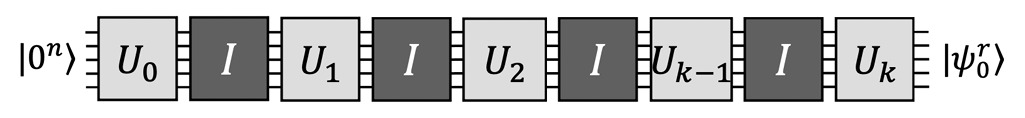
\includegraphics[width=0.75\linewidth]{Images/kqueryIcirc.png}
        \caption{Quantum circuit with $I$ substituted for the $k$ queries}
        \label{fig:kqeryIcirc}
    \end{figure}
    Whenever the identity is substituted into a query gate, we'll call that a blank query. Let's call the final state produced by this $\ket{\psi_0^r}$. That is, $\ket{\psi_0^r}$ is the state that results when the sequence of operations $U_0, U_1,\ldots,U_k$ is carried out, without the oracle operations. Although the superscript $r$ is redundant for this state (because the state is not a function of $r$), it's harmless and it will be convenient to keep this superscript $r$ in our notation. The circuit if figure \ref{fig:kquerycirc} corresponds to the function $f_r$. The circuit in figure \ref{fig:kqeryIcirc} corresponds to the zero function (the function that's zero everywhere).

    What we are going to show is that, for some $r \in \{0,1\}^n$, the Euclidean distance between $\ket{\psi_k^r}$ and $\ket{\psi_0^r}$ is upper bounded as
    \[
    \|\ket{\psi_k^r}-\ket{\psi_0^r}\|\leq \frac{2k}{\sqrt{2^n}}
    \]
    This implies that, if $k$ is asymptotically smaller than $\sqrt{2^n}$ then the bound asymptotically approaches zero. If $\|\ket{\psi_k^r}-\ket{\psi_0^r}\|$ approaches zero then the two states are not distinguishable in the limit. This implies that the algorithm cannot distinguish between $f_r$ and the zero function with constant probability.
    Our goal will be to bound the quantity
    \[
    D_k = \sum_r \|\ket{\psi_k^r}-\ket{\psi_0^r}\|^2
    \]
        Intuitively, $D_k$ is a measure of the deviation after $k$ steps caused by the oracle, from the evolution that would otherwise have ensued. If this quantity is small, then all the states $\ket{\psi_k^r}$ are roughly the same, and it is not possible to correctly identify $x$ with high probability. The strategy of the proof is to demonstrate two things: (a) a bound on $D_k$ that shows it can grow no faster than $\mathcal{O}(k^2)$; and (b) a proof that $D_k$ must be $\Omega(N)$ if it is possible to distinguish $N$ alternatives. Combining these two results gives the desired lower bound. 
    Now let's consider the quantum circuits in figures \ref{fig:kquerycirc} and\ref{fig:kqeryIcirc}, along with some intermediate circuits as shown in figure \ref{fig:kqueryinterm}.
    \begin{figure}[ht]
        \centering
        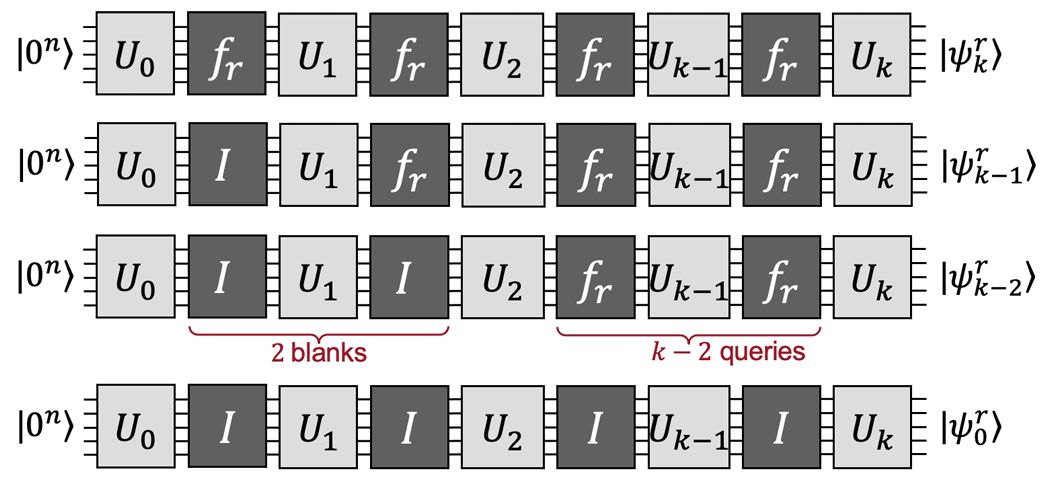
\includegraphics[width=0.75\linewidth]{Images/kqueryinterm.png}
        \caption{Quantum circuits with $i$ blanks, followed by $k-i$ queries to $f_r$ (for $i \in \{0,1,\ldots,r\}$}
        \label{fig:kqueryinterm}
    \end{figure}
    The circuit on top makes all $k$ queries to $f_r$, and recall that we denote the final state that it produces as $\ket{\psi_k^r}$. The next circuit uses the identity in place of the first query and makes the remaining $k-1$ queries to $f_r$. Call the final state of this $\ket{\psi_{k-1}^r}$. The next circuit uses the identity in place of the first two queries and makes the remaining $k-2$ queries to $f_r$. Call the final state that this produces $\ket{\psi_{k-2}^r}$. And continue for $i=3,\ldots,k$ with circuit using the identity in place of the first $i$ queries and then making the remaining $k-i$ queries to $f_r$. Call the final state $\ket{\psi_{k-i}^r}$.

    First, we give an inductive proof that $D_k\leq 4k^2$. This is clearly true for $k=0$, where $D_k=0$. Note that
    \begin{align*}
        D_{k+1}&=\sum_r \|f_r\ket{\psi_k^r} - \ket{\psi_0^r}\|^2\\
        &=\sum_r \|f_r(\ket{\psi_k^r} - \ket{\psi_0^r}) + (f_r -I)\ket{\psi_0^r}\|^2
    \end{align*}
    applying $\|b+c\|^2 \leq \|b\|^2 + \|c\|^2 + 2 \|b\|\|c\|$ with $b\equiv f_r (\ket{\psi_k^r}-\ket{\psi_0^r})$ and $c\equiv (f_r-I)\ket{\psi_k}=-2\braket{x|\psi_k}\ket{x}$, gives
    \[
    D_{k+1} \leq \sum_r (\|\ket{\psi_k^r} - \ket{\psi_0^r}\|^2 + 4|\braket{\psi_k^r|r}|^2 + 4\|\ket{\psi_k^r}-\ket{\psi_0^r}\||\braket{r|\psi_0^r}|)
    \]
    Applying the Cauchy-Schwartz inequality to the second term on the right hand side, and noting that $\sum_r|\braket{x|\psi_0^r}|^2=1$ gives
    \begin{align*}
        D_{k+1} &\leq D_k + 4 \left(\sum_r \|\ket{\psi_k^r} - \ket{\psi_0^r}\|^2\right)^{\frac{1}{2}} \left(\sum_{r'} |\braket{\psi_0^r|r'}|^2\right)^{\frac{1}{2}} + 4\\
        &\leq D_k + 4 \sqrt{D_k} + 4
    \end{align*}
    By inductive hypothesis $D_k \leq 4k^2$ we obtain
    \[
    D_{k+1} \leq 4k^2 + 8k + 4 = 4(k+1)^2
    \]
    which completes the induction.

    To complete the proof we need to show hat the probability of success can only be high if $D_k$ is $\Omega(N)$. We suppose $|\braket{r|\psi_k^r}|^2 \geq 1/2$ for all $r$, so that an observation yields a solution to the search problem with probability at least one-half. Replacing $\ket{x}$ by $e^{\iota \theta}\ket{r}$ does not change the probability of success, so without loss of generality we may assume that $\braket{r|\psi_k^r}=|\braket{r|\psi_k^r}|$, and therefore
    \[
    \|\ket{\psi_k^r}-\ket{\psi_0^r}\|^2 =2-2|\braket{x|\psi_k^x}|\leq 2-\sqrt{2}
    \]
\begin{example}
    Use the Cauchy-Schwarz inequality to show that for any normalized state vector $\ket{\psi}$ and set of $N$ orthonormal basis vectors $\ket{x}$.
    \[
    \sum_x \|\psi-x\|^2 \geq 2N-2\sqrt{N}
    \]
    
\end{example}
    Note that each query where the identity is substituted (blanks query) reveals no information about $r$. Recall that our goal is to show that the $\|\ket{\psi_k^r}-\ket{\psi_0^r}\|$ is small. Notice that we can express the difference between these states as the telescopic sum
    \[
    \ket{\psi_k^r}-\ket{\psi_0^r} = (\ket{\psi_k^r}-\ket{\psi_{k-1}^r}) + (\ket{\psi_{k-1}^r} - \ket{\psi_{k-2}^r}) + \ldots + (\ket{\psi_1^r} - \ket{\psi_0^r})
    \]
    which implies that 
    \[
    \|\ket{\psi_k^r}-\ket{\psi_0^r}\| = \|(\ket{\psi_k^r}-\ket{\psi_{k-1}^r})\| + \|(\ket{\psi_{k-1}^r} - \ket{\psi_{k-2}^r})\| + \ldots + \|(\ket{\psi_1^r} - \ket{\psi_0^r})\|
    \]
    next, we'll upper bound each term $\|\ket{\psi_i^r}-\ket{\psi_{i-1}^r}\|$. To understand the Euclidean distance between $\ket{\psi_i^r}$ and $\ket{\psi_{i-1}^r}$, let's look at the circuits that produce them.
\begin{figure}[ht]
    \centering
    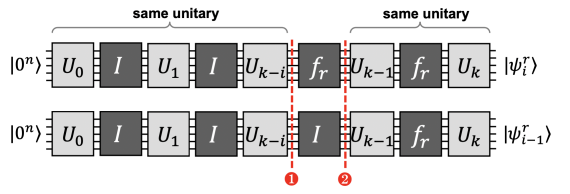
\includegraphics[width=0.75\linewidth]{Images/circuitqueryopt.png}
    \caption{Circuit with $k-i$ blanks and $i$ queries (top) and $k-i+1$ blanks and $i-1$ queries (bottom)}
    \label{fig:circuitqueryopt}
\end{figure}
    Notice that both computations are identical for the first $k-i$ blank queries. We can write the state at state 1 (for both the circuits) as
    \[
    \sum_{x\in\{0,1\}^n} \alpha_{i,x} \ket{x}
    \]
    where of course the state is a unit vector in Euclidean norm (a.k.a, the 2- norm)
    \[
    \sum_{x\in\{0,1\}^n} |\alpha_{i,x}|^2 = 1
    \]
    These states make sense for each $i\in\{1,\ldots,k\}$, and they are independent of $r$.

    It's interesting to consider what happens to the state at the next step .For the bottom computation, nothing happens to the state, since the identity is performed in the query. For the top computation, a query to $f_r$ is performed. Since $f_r$ takes value $1$ only at the point $r$, the $f_r$-query in the phase negates the amplitude of $\ket{r}$ and has no effect on the other amplitudes of the state. Therefore, the state of the top computation at stage 2 is
    \[
    \sum_{x\in\{0,1\}^n}(-1)^{[x=r]} \alpha_{i,x} \ket{x}
    \]
    The difference between the state in the two equations is only in the amplitude of $\ket{r}$, which is negated. So at stage 2 the Euclidean distance between the states of the two circuits is $|\alpha_{r,i}-(-\alpha_{r,i})|=2|\alpha_{r,i}|$.

    Now let's look at what the rest of the two circuits in figure \ref{fig:circuitqueryopt} do. The remaining steps for each circuit are the same unitary operation. Since unitary operations preserve Euclidean distances, this means that
    \[
    \|\ket{\psi_i^r}-\ket{\psi_{i-1}^r}\|=2|\alpha_{i,r}|
    \]
    and this holds for all $i\in\{1,\ldots,k\}$,

    Now consider the average euclidean distance between $\ket{\psi_k^r}$ and $\ket{\psi_0^r}$, averaged over all $n$-bit strings $r$. We can upper bound this as
    \begin{align*}
    \frac{1}{2^n} \sum_{r\in\{0,1\}^n} \|\ket{\psi_k^r}-\ket{\psi_0^r}\|&\leq \frac{1}{2^n} \sum_{r\in\{0,1\}^n} \left(\sum_{i=1}^k \|\ket{\psi_i^r}-\ket{\psi_{i-1}^r}\|\right)\\
    &=\frac{1}{2^n} \sum_{r\in\{0,1\}^n} \left(\sum_{i=1}^k 2|\alpha_{i,r}| \right)\\
    &=\frac{1}{2^n} \sum_{i=1}^k 2\left(\sum_{r\in\{0,1\}^n} |\alpha_{i,r}|\right)\\
    &\leq \frac{1}{2^n} \sum_{i=1}^k 2\left(\sqrt{2^n}\right)\\
    &=\frac{2k}{\sqrt{2^n}}
    \end{align*}
\end{proof}
using the Cauchy-Schwartz inequality, which implies that, for any vector whose $2$- norm is $1$, its maximum possible $1$-norm is the square root of the dimension of the space, which in this case is $\sqrt{2^n}$.

Since an average of Euclidean distances is upper bounded by $2k/\sqrt{2^n}$, there must exist an $r$ for which the Euclidean distance upper bounded by this amount.

Since the denominator is $\sqrt{2^n}$ and the numerate is $2k$, it must be the case that $k$ is proportional to $\sqrt{2^n}$, in order for this Euclidean distance to be a constant. And the Euclidean must be lower bounded by a constant if the algorithm distinguishes between $f_r$ and the zero function with probability $\frac{3}{4}$. This completes the proof that the number of queries $k$ must be order $\sqrt{2^N}$.

This result, that the quantum search algorithm is essentially optimal, is both exciting and disappointing. It is exciting because it tells us that for this problem, at least, we have fully plumbed the depths of quantum mechanics; no further improvement is possible. the disappointment arises because we might have hoped to do much better than the square root speedup offered by the quantum search algorithm. the sort of dream result we might have hoped for a priori is that it would be possible to search an $N$ item search space using $\mathcal{O}(\log N)$ oracle calls/ If such an algorithm existed, it would allows us to solve NP-complete problems efficiently on a quantum computer, since it could search all $2^{\omega(n)}$ possible witnesses using roughly $\omega(n)$ oracle calls, where the polynomial $\omega(n)$ is the length of a witness in bits. Unfortunately, such an algorithm is not possible. This is useful information for would-be algorithm designers, since it indicates that a naive search-based method for attaching NP-complete problems is guaranteed to fail.

Venturing into the real of opinion, we note that many researchers believe that the essential reason for the difficulty of NP-complete problems is that their search space has essentially no structure, and that (up to polynomial factors ) the best possible method for solving such a problem is to adopt a search method. If one takes this point of view, then sit is bad news for quantum computing, indicating that the class of problems efficiently soluble on a quantum computer, BQP does not contain the NP-complete problems. Of course, this is merely opinion, and it is still possible that the NP-complete problems contain some unknown structure that allows them to be efficiently solved on a quantum computer, or perhaps even on a classical computer. A nice example to illustrate this point is the problem of factoring, widely believed to be in the class of NPI problems of intermediate in difficulty between P and NP-complete problems. The key to the efficient quantum mechanical solution of the factoring problem was the exploitation of a structure `hidden' within the problem - structure revealed by the reduction to order-finding. even with this amazing structure revealed, it has not been found possible to exploit the structure to develop an efficient classical algorithm for factoring, although, of course, quantum mechanically the structure can be harnessed to give an efficient factoring algorithm! perhaps a similar structure lurks in other problems b=suspected to be in NPI. such as the graph isomorphism problem, or perhaps even in the NP-complete problems themselves.

\begin{example}
    \textbf{(Optimality for multiple solutions)} Suppose the search problem has $M$ solutions. Show that $\mathcal{O}(\sqrt{N/M})$ oracle applications are required to find a solution.
\end{example}

\subsection{The BBBV Theorem}
It's great that we can get a quadratic speedup with Grover's algorithm, but we were able to get an exponential speedup with Shor's algorithm. So, why can't we get a bigger speedup for unordered search? By now you should have some intuition for the differences between Shor's algorithm and Grover's algorithm. Shor's algorithm provided an exponential speedup by orchestrating a very ``global" phenomenon, involving intereference effect that revealed the period of a black-box periodic function. Grover's algorithm let us turn a little amplitude into a bigger amplitude by adding $\sim \frac{1}{\sqrt{N}}$ with each query. It's faster than classical brute-force search, but still laborious (still needing $\mathcal{O}(\sqrt{N})$ time).

We're still hand-waving this issue though. We haven't rule out the possiblility of a quantum algorithm that beats Grover, solving unordered search in, say $\sqrt[3]{N}$ or $\log (N)$ queries or whatever. For that we need a key result for 1994 called the BBBV Theorem. This theorem is named for Bennett, Bernstein, Brssard and Vazirani, and proved that Grover's algorithm is indeed asymptotically optimal for the black-box unordered search problem.


Note that the BBBV theorem was published in 1994, so it actually predates Grover. Grover's algorithm htus has the rare distincition of being proved to be optimal before it was discovered to exist.

Amusingly, BBBV were trying to prove that there's no magic way to search faster using a quantum computer. They were able to get a lower bound of $\Omega(\sqrt{N})$, and figure that tightening the bound to $\Omega(\sqrt{N})$ was a technicalissue that they could leave for the future - that is, unit Grover cam along and showed why such a tightening is impossible!

While by now we know many proofs of the BBBV Therem, the original (and still most self-contained) proof uses what's called a Hybrid Argument. Imagine we're using an arbitrary quantum algorithm to search for a single marked item in a list of size $N$. Without loss of generality we can say that the algorithm makes a total of $T$ queries and follows some sequence of operations that looks like
\[
U_0\rightarrow Q_0 \rightarrow U_1 \rightarrow Q_1\rightarrow U_2 \rightarrow Q_2 \rightarrow \ldots
\]
where each $Q_t$ is a query and each $U_t$ is some unitary transformation (independent of the data in the list). We start by doing a test run of the algorithm on the all-zero list (without a marked item) and see what happens. What we'll then show is that if we challenge the value of some item in the list from $0$ to $1$ (in other words introduce a marked item), the algorithm won;t notice the change very much. This is done by exploiting the fact that unitary transformations are linear and norm preserving.



\section{Conclusion}
Grover's algorithm  is asymptotically optimal within the query model. It means that it is not possible to come with an algorithm for the search problem (unique or multiple solutions) that uses asymptotically fewer than $\mathcal{O}(\sqrt{n})$ queries in the worst case. This has been proved rigorously and was known even before Grover's algorithm was discovered. This algorithm is broadly applicable as it can be used as a subroutine in other quantum algorithms to use its quadratic speedup on top of other algorithms. The technique used in Grover's algorithm has been generalized and this is called Amplitude Amplification which is then applied to another quantum algorithms to essentially boost its success probability quadratically then it would have been possible classically.

The great utility of this algorithm arises because we do not assume any particular structure to the search problems being performed. This is the great advantage of posing the problem in terms of a `black box' oracle, and we adopt this point of view whenever convenient. In practical applications, of course, it is necessary to understand how the oracle is being implemented, and in each of the practical problems we concern ourselves with an explicit description of the oracle implementation is given. 
\section{Quantum Counting}
How quickly can we determine the number of solutions, $M$, to an $N$ item search problem, if $M$ is not known in advance? Clearly, on a classical computer it takes $\theta(N)$ consultations with an oracle to determine $M$. On a quantum computer it is possible to estimate the number of solutions much more quickly than is possible on a classical computer by combining the Grover iteration with the phase estimation technique based upon the quantum Fourier transform. This has some important applications. First, if we can estimate the number of solutions quickly then it is possible to find a solution quickly, even if the number of solutions is unknown, by first counting the number of solutions, and then applying the quantum search algorithm to find a solution. Second, quantum counting allows us to decide whether or not a solution even exists, depending on whether the number of solutions is zero or non zero. This has applications, for example, to the solution of \textbf{NP}-complete problem, which may be phrased in terms of the existence of a solution to a search problem.

\begin{example}
Consider a classical algorithm for the counting problem which samples uniformly and independently $k$ times from the search space, and let $X_1, \ldots, X_k$ be the results of the oracle calls, that is, $X_j=1$ if the $j$th oracle call revealed a solution to the problem, and $X_j=0$ if the $j$th oracle call did not reveal a solution to the problem. This algorithm returns the estimate $S=N \times \sum_j X_j/k$ for the number of solutions to the search problem. Show that the standard deviation is $\Delta S=\sqrt{a(N-a)/k}$. Prove that to obtain a probability at least $3/4$ of estimating $M$ correctly to within an accuracy $\sqrt{M}$ for all values of $M$ must have $k=\Omega(\sqrt{N})$.
\end{example}
\begin{example}
    Prove that any classical counting algorithm with a probability at least $3/4$ for estimating $M$ correctly to within an accuracy $c\sqrt{M}$ for some constant $c$ and for all values of $M$ must make $\Omega(N)$ oracle calls.
\end{example}

Quantum counting is an application of the phase estimation procedure to estimate the eigenvalues of the grover iteration $G$, which in turn enables us to determine the number of solutions $M$ to the search problem. Suppose $\ket{a}$ and $\ket{b}$ are the two eigenvectors of Grover iteration in the space spanned by $\ket{A}$ and $\ket{B}$. Let $\theta$ be the angle of rotation determined by the Grover iteration. From equation, 
\[
G=\begin{bmatrix} \cos\theta & -\sin \theta \\ \sin \theta & \cos \theta \end{bmatrix}
\]
The characteristic equation is as follows:
\[
\lambda^2 -2\cos \theta \lambda + 1 = 0 
\]
The solutions to these equations are:
\[
\lambda = \frac{2\cos \theta \pm \sqrt{4\cos^2 \theta -1 }}{2} = \cos \theta \pm \sqrt{-\sin^2 \theta} = e^{\iota \theta} , e^{-\iota \theta}
\]
we see that the corresponding eigen values are $e^{\iota \theta}$ and $e^{\iota (2\pi-\theta)}$. For ease of analysis it is convenient to assume that the oracle has been augmented, expanding the size of the search space to $2N$, and ensuring that $sin^2(\theta/2)=a/2N$.

The phase estimation circuit used for quantum counting is as shown in figure \ref{fig:quantumcount}. The function of the circuit is to estimate $\theta$ to $m$ bits of accuracy, with a probability of success at least $1-\epsilon$. The first register contains $t=m+\lceil \log \left(2+1/2\epsilon\right) \rceil$ qubits, as per the phase estimation algorithm, and the second register contains $n+1$ qubits, enough to implement the Grover iteration on the augmented search space. The state of the second register is initialized to an equal superposition of all possible inputs $\sum_x\ket{x}$ by a Hadamard transform. As we saw this state is a superposition of the eigenstates $\ket{a}$ and $\ket{b}$, so the circuit gives us an estimate for $\theta$ or $2\pi-\theta$ accurate to within $|\Delta \theta|\leq 2^{-m}$, with probability at least $1-\epsilon$ with the same level of accuracy, so effectively the phase estimation algorithm determines $\theta$ to an accuracy of $2^{-m}$ with probability $1-\epsilon$.
\begin{figure}[ht]
    \centering
    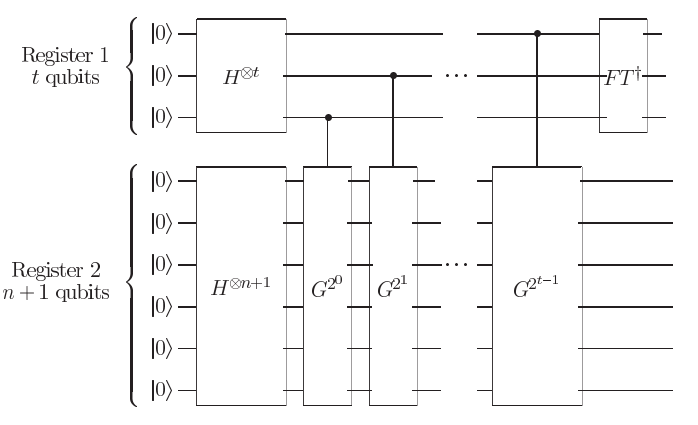
\includegraphics[width=0.75\linewidth]{Images/quantumcounting.png}
    \caption{Circuit for performing approximate quantum counting on a quantum computer}
    \label{fig:quantumcount}
\end{figure}
using the equation $\sin^2(\theta/2)=a/2N$ and our estimate for $\theta$ we obtain an estimate of the number of solutions, a. How large an error, $\Delta M$, is there in this estimate
\begin{align*}
    \frac{|a|}{2N}&=\left|\sin^2\left(\frac{\theta+\Delta \theta}{2}\right) - \sin^2 \left(\frac{\theta}{2}\right)\right|\\
    &=\left(\sin \left(\frac{\theta+\Delta \theta}{2}\right) + \sin \left(\frac{\theta}{2}\right)\right)\left| \sin\left(\frac{\theta+\Delta \theta}{2}\right)-\sin \left(\frac{\theta}{2}\right)\right|
\end{align*}
Calculus implies that $|\sin((\theta+\Delta \theta)-\sin(\theta/2)|\leq |\Delta \theta|/2$, and elementary trigonometry that $|\sin((\theta+\Delta \theta)/2)|\leq \sin(\theta/2)+|\Delta \theta|/2$, so
\[
\frac{|\Delta a|}{2N} < \left(2\sin\left(\frac{\theta}{2}\right) + \frac{|\Delta \theta|}{2}\right)\frac{|\Delta \theta|}{2}
\]
Substituting $\sin^2(\theta/2)=a/2N$ and $|\Delta \theta|\leq 2^{-m}$ gives our final estimate for the error in our estimate of $M$,
\[
|\Delta a| < \left(\sqrt{2aN} + \frac{N}{2^{m+1}}\right)2^{-m}
\]
As an example, suppose we choose $m=\lceil n/2\rceil +1$, and $\epsilon=1/6$. Then we have $t=\lceil n/2\rceil +3$, so the algorithm requires $\Theta(\sqrt{N})$ Grover iterations, and thus $\Theta(\sqrt{N})$ oracle calls. Our accuracy is $|\Delta M|<\sqrt{M/2} + 1/4=\mathcal{O}(\sqrt{M})$. Comparing this with the fact that it would have required $\mathcal{O}(N)$ oracle calls to obtain a similar accuracy on a classical computer.

Indeed, the example just described serves double duty as an algorithm for determining whether a solution to the search problem exists at all, that is, whether $M=0$ or $M\neq 0$. If $M=0$ then we have $|\Delta M|<1/4$, so the algorithm must produce the estimate zero with probability at least $5/6$. Conversely, if $M\neq0$ then it is easy to verify that the estimate for $M$ is not equal to $0$ with probability at least $5/6$.

Another application of quantum counting is to find a solution to a search problem when the number $M$ of solutions is unknown. The difficulty in applying the quantum search algorithm is that the number of time to repeat the Grover iteration, depends on knowing the number of solutions $M$. This problem can be alleviated by using the quantum counting algorithm to first estimate $\theta$ and $M$ to high accuracy using phase estimation, and then to apply the quantum search algorithm, repeating the Grover iteration a number of times determined, with the estimates for $\theta$ and $M$ obtained by the phase estimation substituted to determine $R$. The angular error in this case is at most $\pi/4(1+|\Delta \theta|/\theta)$, so choosing $m=\lceil n/2\rceil +1$ as before gives an angular error at most $\pi/4 \times 3/2=3\pi/8$, which corresponds to a success probability of at least $\cos^2(3\pi/8)=1/2-1/2\sqrt{2}\approx 0.15$ for the search algorithm. If the probability of obtaining an estimate of $\theta$ this accurate is $5/6$. as in our earlier example, then the total probability of obtaining a solution to the search problem is $5/6 \times \cos^2(3\pi/8)\approx 0.12$, a probability which may be boosted close to $1$ by a few repetitions of the combined counting-search procedure.

\section{Amplitude Estimation}
Let $\ket{\psi_0}$ be prepared by an oracle $U_{\psi_0}$ i.e., $U_{\psi_0}\ket{0^n}=\ket{\psi_0}$. We have the knowledge that 
\[
\ket{\psi_0}=\sqrt{p_0}\ket{\psi_{good}} + \sqrt{1-p_0} \ket{\psi_{bad}}
\]
and $p_0 <<1$. Here $\ket{\psi_{bad}}$ is an orthogonal state to the desired state $\ket{\psi_{good}}$, and $\sqrt{p_0}=\sin\frac{\theta}{2}$. The problem of amplitude estimation is to estimate $p_0$ to $\epsilon$-precision. If $p_0$ is away from $0$ or $1$ and is to be estimated directly from the Monte Carlo methods, the number of samples needed is $N=O(\epsilon^{-2})$.

Let $G=R_{\psi_0}R_{good}$ be the grover operator. Then in the basis $B=\{\ket{\psi_{good}},\ket{\psi_{bad}}\}$, the subspace $H=span(B)$ is an invariant subspace of $G$. The matrix representation is
\[
[G]_B =\begin{pmatrix} \cos \theta & \sin \theta \\ - \sin \theta & \cos\theta \end{pmatrix}
\]
Its two eigenstates are
\[
\ket{\psi_{\pm}}=\frac{1}{\sqrt{2}}(\ket{\psi_{good}} \pm \iota \ket{\psi_{bad}})
\]
with the eigenvalues $e^{\pm\theta}$, respectively.

Therefore the problem of estimation $\theta$ can be solved with phase estimation with an imperfect initial state. Note that
\[
|\braket{\psi_0|\psi_{+}}|^2=\frac{1}{2}\left|\sin \frac{\theta}{2} + \iota \cos\frac{\theta}{2} \right|^2 =\frac{1}{2}=|\braket{\psi_0|\psi_{-}}|^2
\]
Consider a QPE circuit with $t$ ancilla qubits and query $G$ for $T=2^t$ times. Then each execution with the system register will be $\ket{\psi_+}$ or $\ket{\psi_{-}}$ states with probability $0.5$. let
\[
t=d+\lceil\log \delta^{-1}\rceil
\]
be the number of ancilla qubits with $\epsilon'=2^{-d}$. Then QPE obtains an estimate denoted by $\tilde{\theta}$, which approximates $\theta$ to precision $\epsilon'$ with success probability $1-\delta$. Note that $p_0=\sin^2\frac{\theta}{2}$, and
\begin{align*}
    &\sin^2 \frac{\tilde{\theta}}{2} - \sin^2 \frac{\theta}{2}\\
    &=\sin^2\frac{\tilde{\theta}-\theta}{2}\cos^2\frac{\theta}{2}+\cos^2\frac{\tilde{\theta}-\theta}{2}\sin^2\frac{\theta}{2}+2\sin\frac{\theta}{2}\cos\frac{\theta}{2}\sin\frac{\tilde{\theta}-\theta}{2}\cos\frac{\tilde{\theta}-\theta}{2}-\sin^2\frac{\theta}{2}\\
    &=\sin\frac{\theta}{2}\cos\frac{\theta}{2}\sin(\tilde{\theta}-\theta)+\left(1-2\sin^2\frac{\theta}{2}\right)\sin^2\frac{\tilde{\theta}-\theta}{2}
\end{align*}
Using the fact that $|\sin(\tilde{\theta}-\theta)|\leq |\tilde{\theta}-\theta|\leq \epsilon'$, we have
\[
|\tilde{p}-p|\leq \sqrt{p_0(1-p_0)}\epsilon' +(1-2p_0)\frac{\epsilon'^2}{4}
\]
Let $\epsilon'$ be sufficiently small. Now if $p_0(1-p_0)=\Omega(1)$, we can choose $\epsilon'=\mathcal{O}(\epsilon)$, and the total complexity of QPE is $\mathcal{O}(\epsilon^{-1})$.

If $p_0$ is small, then we should estimate $p_0$ to multiplicative accuracy $\epsilon$ instead. Use
\[
|\tilde{p}-p|\approx \sqrt{p_0}\epsilon' <p_0\epsilon
\]
we have $\epsilon'=\sqrt{p_0}\epsilon$. Therefore the runtime of QPE is $\mathcal{O}(p_0^{-\frac{1}{2}}\epsilon^{-1})$. If $p_0$ is to be estimated to precision $\epsilon'$ using Monte Carlo methods, the number of samples needed would be $\mathcal{N}=\mathcal{O}(p_0^{-1}\epsilon^{-2})$.

So, the amplitude estimation method achieves quadratic speedup in the total complexity, by the circuit depths is increased to $\mathcal{O}(\epsilon'^{-1}\delta^{-1})$.

\begin{example}
    \textbf{(Amplitude estimation to accelerate hadamard test)} Consider the circuit for the Hadamard test to estimate $Re\bra{\psi}U\ket{\psi}$. Let the initial state $\ket{\psi}$ be prepared by a unitary $U_{\psi}$, then the following combined circuit \ref{fig:acc_hadtest}.
    \begin{figure}[ht]
        \centering
        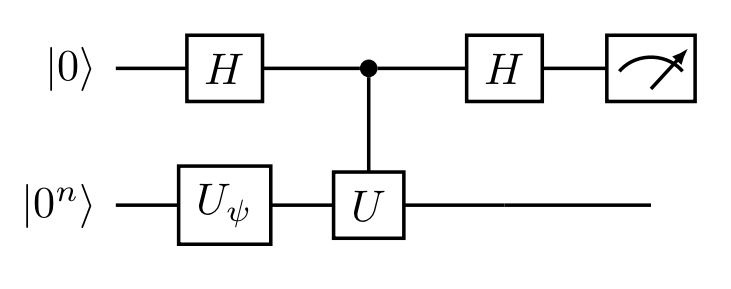
\includegraphics[width=1\linewidth]{Images/Acc_hadamardtest.png}
        \caption{Accelerated Hadamard Test}
        \label{fig:acc_hadtest}
    \end{figure}
    maps $\ket{0}\ket{0^n}$ to
    \[
    \ket{\psi_0}=\frac{1}{2}\ket{0}(\ket{\psi}+U\ket{\psi})+\frac{1}{2}\ket{1}(\ket{\psi}-U\ket{\psi})=\sqrt{p_0}\ket{\psi_{good}}+\sqrt{1-p_0}\ket{\psi_{bad}}
    \]
    and the goal is to estimate $p_0$. This also gives the implementation of the reflector $R_{\psi_0}$.

    Note that $R_{good}$ can be implemented by simply reflecting against the signal qubit, i.e., 
    \[
    R_{good} =(I-2\ket{0}\bra{0})\otimes I_n = -Z\otimes I_n
    \]
    Then we can run QPE to the Grover unitary $G=R_{\psi_0}R_{good}$ to estimate $p(0)$, and the circuit depth is $\mathcal{O}(\epsilon^{-1})$.
\end{example}

\section{Amplitude Amplification}
Grover's algorithm is not restricted to the problem of unstructured search. One immediate application is called amplitude amplification (AA), which is used ubiquitously as a subroutine to achieve quadratic speedups.

Let $\ket{\psi_0}$ be prepared by an oracle $U_{\psi_0}$ i.e. $U_{\psi_0}=\ket{0^n}=\ket{\psi_0}$. We have the knowledge that
\[
\ket{\psi_0}=\sqrt{p_0} \ket{\psi_{good}} + \sqrt{1-p_0}\ket{\psi_{bad}}
\]
and $p_0<<1$. Here $\ket{\psi_{bad}}$ is an orthogonal state to the desired state $\ket{\psi_{good}}$. We cannot get access to $\ket{\psi_{good}}$ directly, but would like to obtain a state that has a large overlap with $\ket{\psi_{good}}$ i.e., amplify the amplitude of $\ket{\psi_{good}}$.

In the problem of unstructured search $\ket{\psi_{good}}=\ket{x_0}$, and $p_0=1/N$. Although we do not have access to the answer $\ket{x_0}$, we assume access to the reflection oracle $R_{x_0}$. Here we also assume access to the reflection oracle
\[
R_{good} = 1-2\ket{\psi_{good}}\bra{\psi_{good}}
\]
From $U_{\psi_0}$, we can construct the reflection with respect to the initial state
\[
R_{\psi_0}=2\ket{\psi_0}\bra{\psi_0} - I=U_{\psi_0}(2\ket{0^n}\bra{0^n}-I)U_{\psi_0}^{\dagger}
\]
via the $n$-qubit controlled-$X$ gate. So following exactly the same procedure as the unstructured search problem, we can construct the Grover iterate
\[
G=R_{\psi_0}R_{good}
\]
Applying $G^k$ to $\ket{\psi_0}$ for some $k=\mathcal{O}(1/\sqrt{p_0})$, we obtain a state that has $\Omega(1)$ overlap with $\ket{\psi_{good}}$.

\begin{example}
    \textbf{(Reflection with respect to signal qubits)} One common scenario is that the implementation of $U_{\psi_0}$ requires $m$ ancilla qubits (also called signal qubits) i.e.,
    \[
    U_{\psi_0}\ket{0^m}\ket{0^n} = \sqrt{p_0}\ket{0^m}\ket{\psi_0}+\sqrt{1-p_0}\ket{\perp}
    \]
    where $\ket{\perp}$ is some orthogonal state satisfying
    \[
    (\Pi \otimes I_n)\ket{\perp}=0; \quad \Pi=\ket{0^m}\bra{0^m}
    \]
    Therefore
    \[
    \ket{\psi_{good}}=\ket{0^m}\ket{\psi_0}
    \]
    This setting is special since the ``good" state can be verified by measuring the ancilla qubits after applying $U_{\psi_0}$, and post-select the outcome $0^m$. In particular, the expected number of measurements needed to obtain $\ket{\psi_{good}}$ is $1/p_0$.

    In order to employ the AA procedure, we first note that the reflection operator can be simplified as
    \[
    R_{good} = (1-2\ket{0^m}\bra{0^m})\otimes I_n = (I-2\Pi)\otimes I_n
    \]
    This is because $\ket{\psi_{good}}$ can be entirely identified by measuring the ancilla qubits. Meanwhile
    \[
    R_{\psi_0}= U_{\psi_0} (2\ket{0^{m+n}}\bra{0^{m+n}}-I)U_{\psi_0}^{\dagger}
    \]
    Let $G=R_{\psi_0}R_{good}$, and applying $G^k$ to $\ket{\psi_0}$ for some $k=\mathcal{O}(1/\sqrt{p_0})$ times, we obtain a state that has $\Omega(1)$ overall with $\ket{\psi_{good}}$. This achieves the desired quadratic speedup.
\end{example}

\begin{example}
    \textbf{(Amplitude Damping)} Assuming access to an oracle, where $p_0$ is large, we can easily dampen the amplitude to any number $\alpha\leq \sqrt{p_0}$. 

    We introduce an additional signal qubit. Then,
    \[
    (I\otimes U_{\psi_0})\ket{0}\ket{0^m}\ket{0^n}=\ket{0}(\sqrt{p_0}\ket{0^m}\ket{\psi_0}+\sqrt{1-p_0}\ket{\perp})
    \]
    Define a single qubit rotation operation as
    \[
    R_{\theta}\ket{0}=\cos \theta\ket{0} + \sin \theta \ket{1}
    \]
    and we have
    \begin{align*}
        &(R_{\theta}\otimes I_{m+n})(I\otimes U_{\psi_0})\ket{0}\ket{0^m}\ket{0^n}\\
        &=\cos\theta \ket{0}(\sqrt{p_0}\ket{0^m}\ket{\psi_0} + \sqrt{1-p_0}\ket{\perp'})+\sin\theta\ket{1}(\sqrt{p_0}\ket{0^m}\ket{\psi_0}+\sqrt{1-p_0}\ket{\perp'})\\
        &=\sqrt{p_0}\cos\theta\ket{0}\ket{0^m}\ket{\psi_0}+\sqrt{1-p_0\cos^2\theta}\ket{\perp'}
    \end{align*}
    Here ($\ket{0^{m+1}}\bra{0^{m+1}}\otimes I_n)\ket{\perp'}=0.$ We only need to choose $\sqrt{p_0}\cos\theta=\alpha$.
\end{example}


\section{Applications of Grover's Algorithm}
\subsection{Application: Satisfiability}
Grover's algorithm has many applications: basically any classical algorithm that has some search component can be improved using Grover's algorithm as a subroutine. This includes many basic computer applications such as finding shortest paths and minimum spanning trees, various other graph algorithms, etc..

We can also use it to speed up the computation of NP-complete problems, albeit only quadratically, not exponentially. As an example, consider the satisfiability problem: we are given a Boolean function $\phi(i_1,\ldots,i_n)$ and want to know if it has a satisfying assignment, i.e., a setting of the bits $i_1,\ldots,i_n$ that makes $\phi(i_1,\ldots,i_n)=1$. A classical brute-force search along all $2^n$ possible assignments takes time roughly $2^n$.

To find a satisfying assignment faster, we define the $N=2^n$-bit input to Grover's algorithm by $x_i=\phi(i)$, where $i\in\{0,1\}^n$. For a given assignment $i=i_1,\ldots i_n$ it is easy to compute $\phi(i)$ classically in polynomial time. We can write that computation as a reversible circuit (using only Toffoli gates), corresponding to a unitary $U_{\phi}$ that maps $\ket{i,0,0}\rightarrow \ket{i,\phi(i),w_i}$, where the third register holds some classical workspace the computation might have needed. To apply grover we need an oracle that puts the answer in the phase and doesn't leave workspace around (as that could mess up the interference effects. Define $O_{x,\pm}\ket{i}=(-1)^{x_i}\ket{i}$; here we did not explicitly write the workspace qubits, which start and end in $\ket{0}$. Now we can run Grover and find a satisfying assignment with high probability if there is one, using a number of elementary operations that is $\sqrt{2^n}$ times some polynomial factor.

If brute-force search is basically the best thing we can do classically to solve some particular NP-hard problem, then that computation can be sped up quadratically on a quantum computer using Grover search like above. However, there are also NP-hard problems where we know algorithms that still run in exponential time, but that are much faster than brute-force search. For example, consider the famous Travelling Salesman Problem (TSP): given an $n$-vertex graph with weights (distances) on the edges, find the shortest tour in this graph that visits every node exactly once. Since there are $(n-1)!$ many different tours, classical brute-force search would take time $(n-1)!$ times some polynomial is $n$. Grover's algorithm could speed this up quadratically. However, there are much more clever classical algorithms for TSP. In particular, Bellman-Held-Karp dynamic programming algorithm solves TSP in time $2^n$, times a polynomial in $n$. This algorithm is much faster than $O(\sqrt{n!})$ (which is roughly $(n/e)^{n/2}$), and is not amenable to a straightforward speed-up using Grover. Nevertheless, it turns out quantum computers can still solve TSP polynomially faster than the best known classical algorithms, albeit in a much more complicated way than by just applying Grover.\cite{ambainis2018quantumspeedupsexponentialtimedynamic}.

\subsection{Speeding up the solutions of NP-complete problems}
Quantum searching may be used to speed up the solution to the problems in the complexity class NP. We already saw, how factoring can be sped up here, we illustrate how quantum search can be applied to assist the solution of the Hamiltonian cycle problem (HC). Recall that a Hamiltonian cycle of a graph is a simple cycle which visits every vertex of the graph. The HC problem is to determine where a given graph has a Hamiltonian cycle or not. This problem belongs to the class of NP-complete problems, widely believed (but not yet proved) to be intractable on a classical computer. A simple algorithm to solve HC is to perform a search through all possible orderings of the vertices:
\begin{enumerate}
    \item Generate each possible ordering $(v_1,\ldots, v_n)$ of vertices for the graph. Repetitions will be allowed, as they ease the analysis without affecting the essential result.
\item For each ordering check whether it is a hamiltonian cycle for the graph. If not, continue checking the orderings.
\end{enumerate}
Since there are $n^n=2^{n\log n}$ possible orderings of the vertices which must be searched for, this algorithm requires $2^{n\log n}$ checks for the Hamiltonian cycle property in the worst case. Indeed, any problem in NP may be solved in a similar way: if a problem of size $n$ has witnesses which can be specified using $\omega(n)$ bits, where $\omega(n)$ is some polynomial in $n$, then searching through all $2^{\omega(n)}$ possible witnesses will reveal a solution to the problem, if one exists.

The quantum search algorithm may be used to speed up this algorithm by increasing the speed of the search. Specifically, we use the algorithm described earlier to determine whether a solution to the search problem exists. Let $m=\lceil \log n\rceil$. The search space for the algorithm will be represented by a string of $mn$ qubits, each block of $m$ qubits being used to store the index to a single vertex. Thus we can write the computational basis states as $\ket{v_1,\ldots,v_n}$, where each $\ket{v_i}$ is represented by the appropriate string of $m$ qubits, for a total of $nm$ qubits. the oracle for the search algorithm must apply the transformation:
\[
O\ket{v_1,\ldots,v_n} = \begin{cases} \ket{v_1,\ldots,v_n}, &\text{if $v_1,\ldots,v_n$ is not a Hamiltonian cycle}\\ -\ket{v_1,\ldots,vn}, &\text{if $v_1,\ldots,v_n$ is a Hamiltonian cycle} \end{cases}
\]
Such an oracle is easy to design and implement when one has a description of the graph. One takes a polynomial size classical circuit recognizing Hamiltonian cycles in the graph and converts it to a reversible circuit, also of polynomial size, computing the transformation $\ket{v_1,\ldots,v_n,q)} \rightarrow \ket{v_1,\ldots,v_n,q\oplus f(v_1,\ldots,v_n)}$, where $f(v_1,\ldots,v_n)=1$ if $(v_1,\ldots,v_n)$ is a Hamiltonian cycle, and is $0$ otherwise. Implementing the corresponding circuit on a quantum circuit with the final qubit starting in the state $(\ket{0}-\ket{1})/\sqrt{2}$ gives the desired transformation. We won't explicitly describe the details here, except to note the key point: the oracle requires a number of gate as polynomial in $n$, as a direct consequence of the fact that Hamiltonian cycles can be recognized using polynomially many gates classically. Applying the variant of the search algorithm which determines whether a solution to the search problem exists. We see that it takes $O(2^{mn/2})=O(2^{n\lceil \log n\rceil/2})$ applications of the oracle to determine whether a Hamiltonian cycle exists. When one does exist it is easy to apply the combined counting-search algorithm to find an example of such a cycle, which can be exhibited as a witness for the problem.

To summarize:
\begin{itemize}
    \item The classical algorithm requires $)(p(n)2^{n\lceil \log n\rceil})$ operations to determine whether a Hamiltonian cycle exists, where the polynomial factor $p(n)$ is overhead predominantly due to the implementation of the oracle, that is, the gates checking whether a candidate paths is Hamiltonian or not. The dominant effect in determining the resources requires is the exponent in $2^{n\lceil \log \rceil})$. The classical algorithm is deterministic, that is, it succeeds with probability $1$.
    \item the quantum algorithm requires $)(p(n)2^{n\lceil \log n\rceil/2})$ operations to determine whether a Hamiltonian cycle exists. Once again, the polynomial $p(n)$ is overhead predominantly due to implementation of oracle. the dominant effect in determining the resources requires is the exponent in $2^{n\lceil \log n\rceil/2}$. There is a constant probability (say, $1/6$) of error for the algorithm, which may be reduced to $1/6^r$ by $r$ repetitions of the algorithm.
    \item Asymptotically the quantum algorithm requires the square root of the number of operations the classical algorithm requires.
\end{itemize}








\subsection{Quantum Search of an unstructured database}
Suppose somebody gives you a list containing one thousand flower names, and asks you where `Peth Rose' appears on the list. If the flower appears exactly once on the list, and the list is not ordered in any obvious way, then you will need to examining five hundred names, on average, before you find the `Peth Rose'. Might it be possible to speed up this king of database searching using the quantum search algorithm? Indeed, the quantum search algorithm is sometimes referred to as a database search algorithm, but its usefulness for that application is limited, and based on certain assumptions. In this section we take a look at how the quantum search algorithm can conceptually be used to search an unstructured database, in a setting rather like that found on a conventional computer. The picture we construct will clarify what resources are required to enable a quantum computer to search classical databases.

Suppose we have a database containing $N=2^n$ items, each of length $l$ bits. We will label these items $d_1,\ldots,d_N$. We want to determine where a particular $l$ bit string, $s$, is in the database. A classical computer, used to solve this problem, is typically split into two parts, illustrated in figure \ref{fig:splitcpuparts}. One is the central processing unit, or CPU, where data manipulation takes place, using a small amount of temporary memory. The second part is a large memory which stores the database in a string of $2^n$ blocks of $l$ bit cells. The memory is assumed to be passive, in the sense that it is not capable of processing data on its own. What is possible is to LOAD data from memory into the CPU, and store data from the CPU in memory, and to do manipulations of the data stored temporarily in the CPU. Of course, the classical computers may be designed along different lines, but this CPU-memory split is a popular common architecture.
\begin{figure}[ht]
    \centering
    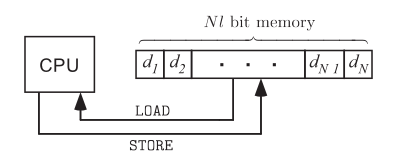
\includegraphics[width=0.75\linewidth]{Images/splitcpuparts.png}
    \caption{Classical Database searching on a computer with distinct central processing unit (CPU) and memory. Only two operations may be directly performed on the memory - a memory element may be LOADed into the CPU, or an item from the CPU may be STOREd in memory}
    \label{fig:splitcpuparts}
\end{figure}
To find out where a given string $s$ is in the unstructured database, the most efficient classical algorithm is as follows. First, an $n$ bit index to the database elements is set up in the CPU. We assume that the CPU is large enough to store the $n=\lceil \log N\rceil $ bit index. The index starts out at zero, and is incremented by one on each iteration of the algorithm. At each iteration, the database entry corresponding to the index is loaded into the CPU, and compared to the string which is being searched for. If they are the same, the algorithm outputs the value of the index and halts. If not, the algorithm continues incrementing the index. Obviously, this algorithm requires that items be loaded from memory $2^n$ times in the worst case. It is also clerar that this is the most efficient possible algorithm for soloving the proble in this model of computation.

How efficiently can an analogous algorithm be implemented on a quantum computer? And, even if a quantum speedup is possible, how useful is such an algorithm? We show first that a speedup is possible, and then return to the question of the utility of such an algorithm. Suppose our quantum computer consists of two units, just like the classical computer, a CPU and a memory. We assume that the CPU contains four registers (1) an $n$ qubit `index' register initialized to $\ket{0}$; (2) an $l$ qubit register initialized to $\ket{s}$ and remaining in that state for the entire computation; (3) an $l$ qubit `data' register initialized to $\ket{0}$; and (4) a $1$ qubit register initialized to $(\ket{0}-\ket{1})/\sqrt{2}$.

The memory unit can be implemented in one of two ways. The simplest is a quantum memory containing $N=2^n$ cells of $l$ qubits, each, containing the database entries $\ket{d_x}$. The second implementation is to implement the memory as a classical memory with $N=2^n$ cells of $l$ bits each, containing the database entries $d_x$. Unlike a traditional memory, however, tit can be addressed by an index $x$ which can be in a superposition of multiple values. This quantum index allows a superposition of cell values to be LOADed from memory. Memory access works in the following way: if the CPU's index register is in the state $\ket{x}$ and the data register is in the state $\ket{d}$, then the contents $d_x$ of the $x$th memory cell are added to the data register $:\ket{d} \rightarrow \ket{d \oplus d_x}$, where the addition is done bitwise, modulo $2$. First, let us see how this capability is used to perform quantum search, then we shall discuss how such a memory might be physically constructed.

The key part of implementing quantum search algorithm is realization of oracle, which must flip the phase of the index which locates $s$ in the memory. Suppose the CPU is in the state 
\[
\ket{x}\ket{s}\ket{0}\frac{\ket{0}-\ket{1}}{\sqrt{2}}
\]
Applying the LOAD operation puts the computer in the state
\[
\ket{x}\ket{s}\ket{d_x}\frac{\ket{0}-\ket{1}}{\sqrt{2}}
\]
Now the second and third registers are compared and if they are the same, then a bit flip is applied to register $4$; otherwise nothing is changed. The effect of this operation is 
\[
\ket{x}\ket{s}\ket{d_x}\frac{\ket{0}-\ket{1}}{\sqrt{2}}\rightarrow \begin{cases} -\ket{x}\ket{s}\ket{d_x}\frac{\ket{0}-\ket{1}}{\sqrt{2}}, &\text{if $d_x=s$}\\
\ket{x}\ket{s}\ket{d_x}\frac{\ket{0}-\ket{1}}{\sqrt{2}}, & \text{if $d_x\neq s$} \end{cases}
\]
The data register is then restored to the state $\ket{0}$ by performing the LOAD operation again. The total action of the oracle thus leaves registers $2,3$ and $4$ unaffected, and unentangled with register $1$ from $\ket{x}$ to $-\ket{x}$ if $d_x=s$, and to leave the register alone otherwise. Using the oracle implemented in this way, we may apply the quantum search algorithm to determine the location of $s$ in the database, using $\mathcal{O}(\sqrt{N})$ LOAD operations, compared to the $N$ LOAD operations required classically.

In order for the oracle to function correctly on superpositions it seems at first glance as though the memory needs to be quantum mechanical. In fact,as we noted above, with some caveats the memory can actually be implemented classically, which likely makes it much more resistant to the effects of noise. But a quantum addressing scheme is still needed; a conceptual picture illustrating how this might be done is shown in figure \ref{fig:unstructdbs}. The principle of operation is a means by which the binary encoded state of the quantum index (where $0$ to $2^n-1$ is represented by $n$ qubits) is translated into a unary encoding (where $0$ to $2^n-1$ is represented by the position of a single problem within $2^n$ possible locations) which address the classical database. The database effects a change on a degree of freedom within the problem which is unrelated to its position. The binary to unary encode is then reversed, leaving the data register with the desire contents.

Are there practical instances in which the quantum search algorithm could be useful for searching classical databases? Two distinct points can be made. First, databases are not ordinarily unstructured. Simple databases, like one containing flower names discussed in the introduction of this section, may be maintained in alphabetical order, such that a binary search can be used to locate an item in time which is $\mathcal{O}(\log (N))$ for an $N$-element database. However, some databases may require a much more complex structure, and although sophisticated techniques exist to optimize classical searches, given queries of a sufficiently complex of unanticipated nature, a predetermined structure may not be of assistance, and the problem can be regarded as being essentially the unstructured search problem as we discussed.

Second, for a quantum computer to be able to search. classical database, a quantum addressing scheme is required. The scheme we depicted requires $\mathcal{O}(N\log N)$ quantum switches about the same amount of hardware as would be required to store the database itself. Presumably, these switches may some day be as simple and inexpensive as classical memory elements, but if that is not the case, then building a quantum computer to perform quantum search may not be economically advantageous, compared with using classical computing hardware distributed over the memory elements,

Given these considerations, it appears that the principle of quantum search algorithms will not be in searching classical databases. Rather, their use will probably be in searching for solutions to hard problems such as the Hamiltonian cycle, traveling salesman, and satisfiability problems.

\begin{figure}[ht]
    \centering
    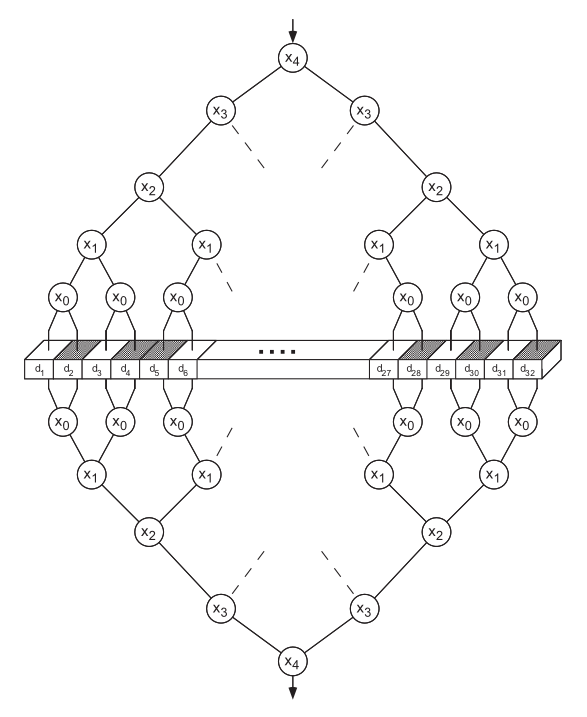
\includegraphics[width=0.5\linewidth]{Images/databaseunstruct.png}
    \caption{Conceptual diagram of a 32 cell classical memory with a five qubit quantum addressing scheme. Each circle represents a switch, addressed by the qubit inscribed within. For example, when $\ket{x_4}=\ket{0}$, the corresponding switch routes the input qubit towards the left; when $\ket{x_4}=\ket{1}$ the switch routes the input qubit to the right. IF $\ket{x_4}=(\ket{0}+\ket{1})/\sqrt{2}$, then an equal superposition of both routes is take. The data register qubits enter at the top of the tree, and are routed down to the database, which changes their state according to the contents of the memory. The qubits are then routed back into a definite position, leaving them with the retrieved information. Physically, this could be realized using, for example, single photons, for the data register qubits, which are steered using nonlinear interferometers. The classical database could be just a simple sheet of plastic in which a `zero' (illustrated as white squares) transmits light unchanged, and a `one' (shaded squares) shifts polarization of the incident light by $90 ^{\circ}$}
    \label{fig:unstructdbs}
\end{figure}


\subsection{The Collision Problem}
In the simplest version of the so-called Collision problem, we're given quantum black-box oracles access to a function $f:\{1,\ldots,N\}\rightarrow \{1,\ldots,N\}$, where $N$ is even, and we're promised that $f$ is two-to-one. The problem is to find $x$ and $y$ such that $x\neq y$ and $f9x)=f(y)$. Since $f$ is two-to-one, there are lots of collisions to be found and the challenge is just to find one of them. In another version of this problem, we're promised that either $f$ is one-to-one or it's two-to-one, and the problem is to decide which. Clearly if we could solve the search version then we could also solve the decision version, by simply outputting that $f$ is two-to-one if a collision is found or that $f$ is one-to-one if not. Conversely, any lower bound for the decision version implies the same lower bound for the search version (but there's no obvious reduction in the other direction).
The collision problem often arises in cryptography when we're trying to break collision resistant hash functions. You can think of the collision problem as being a lot like Simon's problem but with less structure or alternatively, as being like the Grover search problem but with more structure.

With a classical randomized algorithm given black-box access to $f$, $\Theta(\sqrt{N})$ queries are necessary and sufficient to solve the collision problem. Why? The upper bound follows from the famous ``birthday attack". If there are $N$ days in the year, then you only need to ask about $\sqrt{N}$ people before there's an excellent chance that you'll find two with the same birthday. This is because what matters is the number of pairs of people, which grows quadratically with the number of people asked. The lower bound can be proven using the union bound, With a random two-to-one function, each pair has only $a\sim \frac{1}{N}$ .

\section{Implementation using Qiskit}
\subsection{Background}
Usage estimate: 4 seconds (NOTE; This is an estimate only. Your runtime may vary)\\
Amplitude amplification is a general purpose quantum algorithm, or subroutine, that can be used to obtain a quadratic speedup over a handful of classical algorithms. Grover's algorithm was the first to demonstrate this speedup on unstructured search problems. Formulating a Grover's search problem requires an oracle function that marks one or more computational basis states as the states we are interested in finding, and an amplification circuit that increase the amplitude of marked states, consequently suppressing the remaining states.

Here, we demonstrate how to construct Grover oracles and use the \textit{GroverOperator} from the Qiskit circuit library to easily set up a Grover's search instance. The runtime \textit{Sampler} primitive allows seamless execution of Grover circuits.

\subsection{Requirements}
Before starting this tutorial, enusre that you have the following installed:
\begin{itemize}
    \item Qiskit SDK 1.0 or later, with visualization support ( pip install 'qiskit[visualization]')
    \item Qiskit Runtime (pip install qiskit-ibm-runtime) 0.22 or later
\end{itemize}

\subsection{Setup}
Here we import the small number of tools we need for this tutorial.
\begin{lstlisting}[language=Python]
# Built-in modules
import math

# Imports from Qiskit
from qiskit import QuantumCircuit
from qiskit.circuit.library import GroverOperator, MCMT, ZGate
from qiskit.visualization import plot_distribution

# Imports from Qiskit Runtime
from qiskit_ibm_runtime import QiskitRuntimeService
from qiskit_ibm_runtime import SamplerV2 as Sampler
\end{lstlisting}
\begin{lstlisting}[language=Python]
# To run on hardware, select the backend with the fewest number of jobs in the queue
service = QiskitRuntimeService(channel="ibm_quantum")
backend = service.least_busy(operational=True, simulator=False)
backend.name
\end{lstlisting}
This output one of the ibm quantum computers (say 'ibm\_kyoto').
\begin{enumerate}
    \item \textbf{Step 1: Map classical inputs to a quantum problem}: \\
    Grover's algorithm requires an oracle that specifies one or more marked computational basis states, where "marked" means a state with a phase of -1, A controlled-Z gate, or its multi-controlled generation over N qubits, marks the $2^N-1$ state ('1' * N bit-string). Marking basis states with one or more '0' in the binary representation requires applying X-gates on the corresponding qubtis before and after the controlled-Z gate; equivalent to having an open-control on that qubit. In the following code, we define an oracle tht does just that, marking one or more input basis states defined through their bit-string representation. The MCMT gate is used to implement the multi-controlled Z gate.
    \begin{lstlisting}[language=Python]
def grover_oracle(marked_states):
"""Build a Grover oracle for multiple marked states

Here we assume all input marked states have the same number of bits

Parameters:
    marked_states (str or list): Marked states of oracle

Returns:
    QuantumCircuit: Quantum circuit representing Grover oracle
"""
if not isinstance(marked_states, list):
    marked_states = [marked_states]
# Compute the number of qubits in circuit
num_qubits = len(marked_states[0])

qc = QuantumCircuit(num_qubits)
# Mark each target state in the input list
for target in marked_states:
    # Flip target bit-string to match Qiskit bit-ordering
    rev_target = target[::-1]
    # Find the indices of all the '0' elements in bit-string
    zero_inds = [ind for ind in range(num_qubits) if rev_target.startswith("0", ind)]
    # Add a multi-controlled Z-gate with pre- and post-applied X-gates (open-controls)
    # where the target bit-string has a '0' entry
    qc.x(zero_inds)
    qc.compose(MCMT(ZGate(), num_qubits - 1, 1), inplace=True)
    qc.x(zero_inds)
return qc
    \end{lstlisting}
    \textbf{Specific Grover's Instance}\\
Now that we have the oracle function, we can define a specific instance of Grover search. In this example we will mark two computational state out of the eight available in a three-qubit computational space:
\begin{lstlisting}[language=Python]
marked_states = ["011", "100"]

oracle = grover_oracle(marked_states)
oracle.draw(output="mpl", style="iqp")
\end{lstlisting}
This output is as shown in the following figure \ref{fig:grover_tut_markedstates}
\begin{figure}[ht]
    \centering
    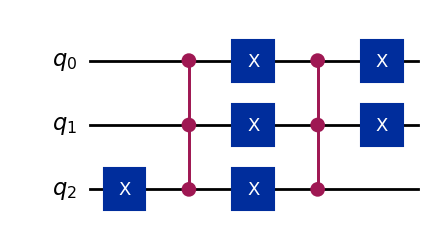
\includegraphics[width=0.5\linewidth]{Images/grover_tut_markedstates.png}
    \caption{Specific Grover's Instance}
    \label{fig:grover_tut_markedstates}
\end{figure}
\textbf{GroverOperator}\\
The built-in Qiskit GroverOperator takes an oracle circuit and returns a circuit that is composed of the oracle circuit and a circuit that amplifies the states marked by the oracle. Here, we decompose the circuit to see the gates within the operator:
\begin{lstlisting}[language=Python]
grover_op = GroverOperator(oracle)
grover_op.decompose().draw(output="mpl", style="iqp")
\end{lstlisting}
This outputs as shown in the figure \ref{fig:grover_op}.
\begin{figure}[ht]
    \centering
    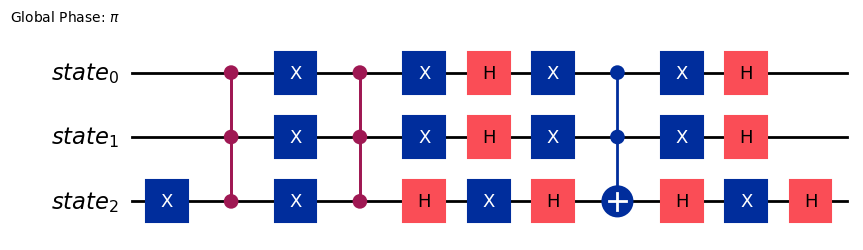
\includegraphics[width=0.6\linewidth]{Images/grover_op.png}
    \caption{Grover Operator}
    \label{fig:grover_op}
\end{figure}
Repeated application of this grover\_op circuit amplify the marked states, making them the most probable bit-strings in the output distribution from the circuit. There is an optimal number of such application that is determined by the ratio of marked states to the total number of possible computational states:
\begin{lstlisting}[language=Python]
optimal_num_iterations = math.floor(
math.pi / (4 * math.asin(math.sqrt(len(marked_states) / 2**grover_op.num_qubits)))
)
\end{lstlisting}
\textbf{Full grover circuit\\}
A complete Grover experiment starts with a Hadamard gate on each qubit; creating an even superposition of all computational basis states, followed the Grover operator (grover\_op) repeated the optimal number of times. Here we make use of the QuantumCircuit.power(INT) method to repeatedly apply the Grover operator.
\begin{lstlisting}[language=Python]
qc = QuantumCircuit(grover_op.num_qubits)
# Create even superposition of all basis states
qc.h(range(grover_op.num_qubits))
# Apply Grover operator the optimal number of times
qc.compose(grover_op.power(optimal_num_iterations), inplace=True)
# Measure all qubits
qc.measure_all()
qc.draw(output="mpl", style="iqp")
\end{lstlisting}
This output the following figure \ref{fig:grover circuit}
\begin{figure}[ht]
    \centering
    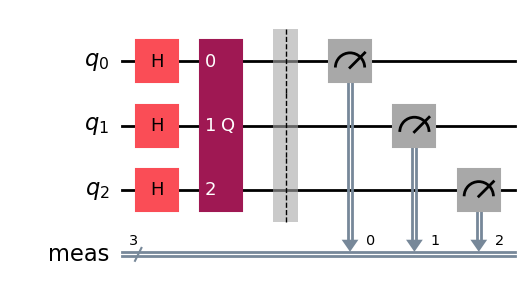
\includegraphics[width=0.6\linewidth]{Images/grover_circuit.png}
    \caption{Full Grover Circuit}
    \label{fig:grover circuit}
\end{figure}
\item \textbf{Step 2: Optimize problem for Quantum Execution}\\
\begin{lstlisting}[language=Python]
from qiskit.transpiler.preset_passmanagers import generate_preset_pass_manager

target = backend.target
pm = generate_preset_pass_manager(target=target, optimization_level=3)

circuit_isa = pm.run(qc)
circuit_isa.draw(output="mpl", idle_wires=False, style="iqp")
\end{lstlisting}
This outputs the following \ref{fig:grover_step2_optimize}.
\begin{figure}[ht]
    \centering
    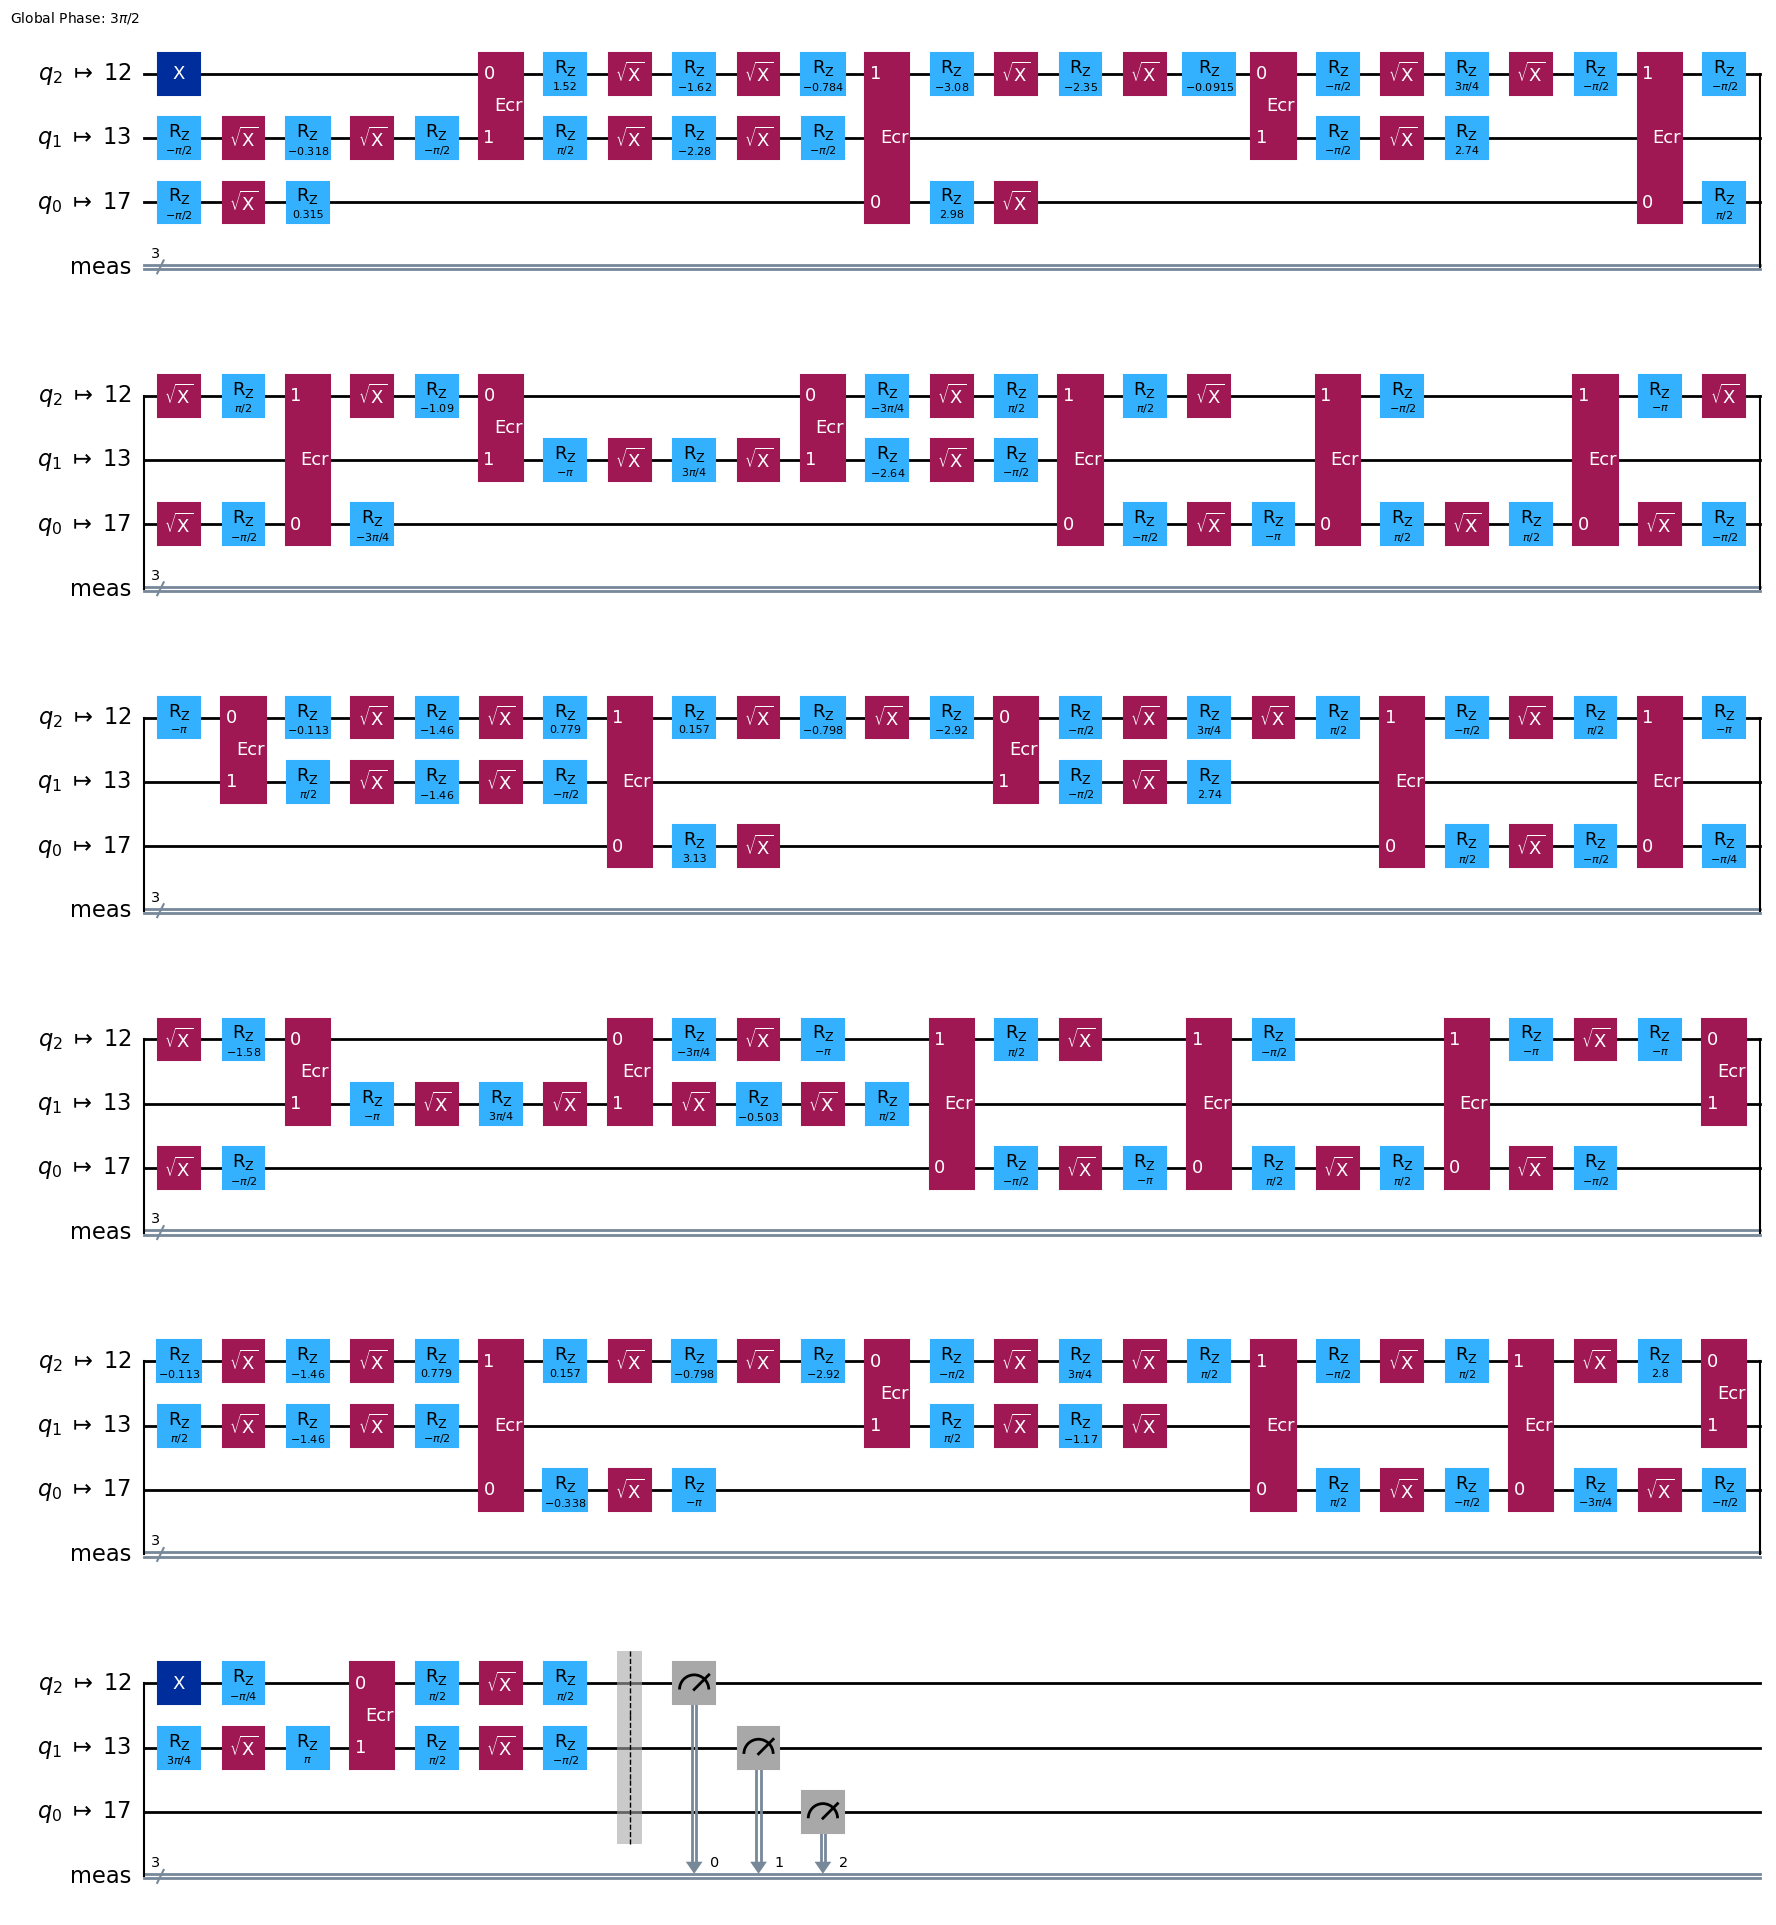
\includegraphics[width=0.6\linewidth]{Images/grover_step2_optimize.png}
    \caption{Optimized Circuit}
    \label{fig:grover_step2_optimize}
\end{figure}
\item \textbf{Step 3: Execute using Qiskit Primitives}\\
Amplitude amplification is a sampling problem that is suitable for execution with the Sampler runtime primitive.

Note that the run() method of Qiskit Runtime SampleV2 takes an iterable of primitive unified blocs (PUBs). For sampler, each PUB is an iterable in the format (circuit, parameter\_values). However, at a minimum, it takes a list of quantum circuit(s).
\begin{lstlisting}[language=Python]
# To run on local simulator:
#   1. Use the SatetvectorSampler from qiskit.primitives instead
sampler = Sampler(backend=backend)
sampler.options.default_shots = 10_000
result = sampler.run([circuit_isa]).result()
dist = result[0].data.meas.get_counts()    
\end{lstlisting}
\item \textbf{Step 4: Post-Process, return result in classical format}\\
\begin{lstlisting}[language=Python]
plot_distribution(dist)
\end{lstlisting}
The result upon measurement is as shown in the figure \ref{fig:grover_results}
\begin{figure}[ht]
    \centering
    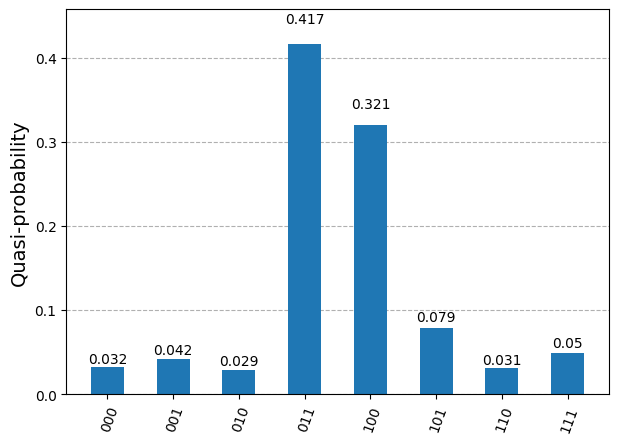
\includegraphics[width=0.7\linewidth]{Images/grover_result.png}
    \caption{Probability plot}
    \label{fig:grover_results}
\end{figure}
\end{enumerate}

